\documentclass{cmspaper}
\usepackage{graphicx}
\usepackage{rotate}
\usepackage{relsize}
\newcommand{\met} {\ensuremath{E\!\!\!\!/_T}}
\newcommand{\ttbar} {\ensuremath{t\bar{t}~}}
\newcommand{\ptll} {\ensuremath{P_T(\ell\ell)}}
\newcommand{\ptllres} {\ensuremath{P^{\rm res}_T(\ell\ell)}}

\begin{document}

%==============================================================================
% title page for many authors
%
\begin{titlepage}
\title{Data driven background study for new physics searches with same sign dileptons at $\sqrt{s} = 10 $ TeV}

  \begin{Authlist}
    D.~ Barge, C.~Campagnari, P.~Kalavase, D.~Kovalskyi, V.~Krutelyov, J.~Ribnik
    \Instfoot{ucsb}{University of California, Santa Barbara}
    W.~Andrews, D.~Evans, F.~Golf, J.~M\"ulmenst\"adt, S.~Padhi, Y.~Tu, F.~W\"urthwein, A.~Yagil
    \Instfoot{ucsd}{University of California, San Diego}
    L.~Bauerdick, I.~Bloch, K.~Burkett, I.~Fisk, O.~Gutsche
    \Instfoot{fnal}{Fermi National Accelerator Laboratory, Batavia, Illinois}
  \end{Authlist}

\begin{abstract}
We discuss data driven methods to estimate the number of same sign Standard Model dilepton
events in searches for new physics characterized by large \met~ and significant hadronic
activity.  For these searches, the dominant background is from \ttbar events. The study 
provides a new method to estimate the charge mis-measurement of leptons. The residual
flavor enriched background is estimated using the lepton fake rate method. We show sensitivity to  
several SUSY benchmark points using 100 pb$^{-1}$ of integrated luminosity.
\end{abstract}
\end{titlepage}

\section{Introduction}
\label{sec:intro}

After the successful operation of the Large Hadron Collider (LHC) and the CMS detector
in 2010 and 2011, and with good prospects for the future, the LHC is now ready to shed light on a number 
of open questions in Particle Physics 
such as the mechanism of electroweak (EW) symmetry breaking, or the 
new physics, Beyond the Standard Model (BSM), that stabilizes the EW scale. 

A wealth of theories that extend the Standard Model have been put forth during the past decades. Supersymmetry (SUSY) is
arguably the best motivated BSM theory --- and certainly the most 
thoroughly studied. 
Indeed, searches for SUSY are among the primary objectives of the 
CMS experiment. SUSY is exceedingly popular not 
only for its theoretical beauty but also because SUSY phenomenology 
is extremely rich, 
%in fact is can mimic almost any other new physics scenario. 
leading to a large variety of possible new signals at the LHC. 
In spite of this, the majority of SUSY studies focus on a very special 
setup: the so-called Constrained Minimal Supersymmetric Standard Model (CMSSM). 
This was justified in the preparation for discoveries as the CMSSM, 
having just a handful of new parameters, is very predicive. However, 
the simplifying assumption of universality at the GUT scale lacks a sound 
theoretical motivation. Consequently, the CMSSM should be regarded as a showcase 
model. When it comes to interpreting experimental results, it is reasonable and interesting to do this within the CMSSM because it 
provides (to some degree) an easy way to show performances, 
compare limits or reaches, etc. However, the interpretation of experimental results in the 
$(m_0,m_{1/2})$ plane risks imposing unwarranted constraints on SUSY, as many 
mass patterns and signatures that are possible a priori are not covered in the CMSSM. 
The same problem arises in any analysis that assumes a particular 
SUSY breaking scheme. 

In this document, we therefore introduce a different approach, which uses only 
minimal assumptions on the underlying SUSY parameters. In particular, given the absence of experimental guidance, we choose
not to rely on a particular SUSY breaking scheme.
Instead, we use a 19-dimensional 
parametrization of the MSSM, called the \emph{phenomenological MSSM} (pMSSM),
with parameters defined not at the GUT scale but instead at the SUSY scale 
(by convention the geometric mean of the two stop masses).
We demonstrate the feasibility of our approach by applying it to 
the 2011 CMS data-set corresponding to 1~fb$^{-1}$ of integrated luminosity.  
Using profile likelihoods, we combine 
the dijet $\alpha_T$ analysis, the opposite-sign dilepton 
analysis and the same-sign dilepton analysis and derive constraints 
on the SUSY particles with as few simplifying assumptions as possible.
Results from other SUSY analyses in CMS will be added as soon as they become available.

We first give the motivation to go beyond the CMSSM and work in 
a generic MSSM setup. After this, the pMSSM and its parametrization is defined. 
We then outline our analysis, giving details on the pMSSM points we have used, 
the detector simulation and the CMS analyses, and describe the statistical method based on 
profile likelihoods used for coping with the 19-dimensional model. Finally, we discuss our results and summarize our conclusions.


\section{Data Samples}
\label{sec:datasamples}
This study is based on the 2\_2\_X re-reco full simulation data samples
listed in Table~\ref{tab:datasets}.  The Standard Model (SM) data sets have been normalized 
to the cross-sections compiled by the top group~\cite{tosi};  for the SUSY 
data sets we used the cross-sections from the Summer 2008 production 
page~\cite{summer08}.

\begin{table}[hbt]
\begin{center}
\begin{tabular}{|l|}\hline
{\tt /TTJets-madgraph/Fall08\_IDEAL\_V11\_redigi\_v10/GEN-SIM-RECO} \\
{\tt /WJets-madgraph/Summer08\_IDEAL\_V11\_redigi\_v1/GEN-SIM-RECO} \\
{\tt /ZJets-madgraph/Summer08\_IDEAL\_V11\_redigi\_v1/GEN-SIM-RECO} \\
{\tt /WW/Summer08\_IDEAL\_V11\_redigi\_v1/GEN-SIM-RECO} \\
{\tt /WZ\_incl/Summer08\_IDEAL\_V11\_redigi\_v1/GEN-SIM-RECO} \\
{\tt /ZZ/Summer08\_IDEAL\_V11\_redigi\_v1/GEN-SIM-RECO} \\
{\tt /SingleTop\_sChannel/Summer08\_IDEAL\_V11\_redigi\_v3/GEN-SIM-RECO} \\
{\tt /SingleTop\_tWChannel/Summer08\_IDEAL\_V11\_redigi\_v3/GEN-SIM-RECO} \\
{\tt /SingleTop\_tChannel/Summer08\_IDEAL\_V11\_redigi\_v3/GEN-SIM-RECO} \\
{\tt /SUSY\_LM0-sftsht/Summer08\_IDEAL\_V11\_v1/GEN-SIM-RECO} \\
{\tt /SUSY\_LM*-sftsht/Summer08\_IDEAL\_V11\_redigi\_v1/GEN-SIM-RECO} \\
\hline
\end{tabular}
\caption{The data sets used in this study.\label{tab:datasets}}
\end{center}
\end{table}

Monte Carlo events were analyzed with CMSSW\_2\_2\_10 
with the additional tags listed in Table~\ref{tab:tags}.

\begin{table} [htb]
\begin{center} 
\begin{tabular}{|l|} \hline
{V01-08-04 CondFormats/JetMETObjects} \\
{V00-06-02-09 DataFormats/METReco} \\
{V07-02-12-03 DataFormats/MuonReco} \\
{V01-08-02-01 JetMETCorrections/Algorithms} \\
{V01-08-15 JetMETCorrections/Configuration} \\
{V03-02-06 JetMETCorrections/JetPlusTrack} \\
{V02-09-02 JetMETCorrections/Modules} \\
{VB04-00-02-04 JetMETCorrections/Type1MET} \\
{V01-04-03 RecoJets/JetAssociationAlgorithms} \\
{V00-04-02-17 RecoMET/Configuration} \\
{V02-05-00-21 RecoMET/METAlgorithms} \\
{V02-08-02-17 RecoMET/METProducers} \\
{V03-26-04 DataFormats/PatCandidate} \\
{V05-05-09 PhysicsTools/PatAlgos} \\
{V03-06-03 PhysicsTools/PatUtils} \\
{V03-01-16 PhysicsTools/PFCandProducer} \\
{V09-30-03 PhysicsTools/HepMCCandAlgos} \\
{V05-13-02 DataFormats/HepMCCandidate} \\
\hline
\end{tabular}
\caption{Additional software tags used in this study.\label{tab:tags}}
\end{center}
\end{table}

\section{Event Selection}
\label{sec:eventselection}

The event selection used is not optimized for any specific non-standard model 
scenario. It is based on small modifications to the baseline 
di-lepton event selection that we used in our same-sign published study~\cite{ssnote1, sspaper}. The 
only difference is that we now require both leptons to have the transverse 
momentum ($p_t$) $> 20$ GeV. A quick summary of the event selection is:

\begin{itemize}
\item We require a mixture of unprescaled single and double lepton triggers as mentioned in~\cite{ssnote1}.
 The combined trigger efficiency is $\sim 99.9 \pm 0.1$\% for di-lepton events that pass the event selection.
\item At least two isolated same sign leptons ($ee$, $e\mu$, and $\mu\mu$). 
\item Leptons must have $P_T > 20$ GeV, $|\eta|< 2.4$.
\item We consider L2L3 corrected particle flow Jets with $P_T > 30$ GeV and
	$|\eta|< 2.4$.
\item The scalar sum of the $P_T$ of all jets passing the requirements above should be $>$ 60 GeV.
\item At least two jets.
\item We remove di-lepton events with invariant mass $ < 5$ GeV.

\item Additional Z-Veto:
\begin{itemize}
      \item  we veto the candidate lepton, if an extra lepton in the event pairs with the candidate lepton
             to form a $Z$ within the mass range between $76 < m_{\ell\ell} $ (GeV) $< 106$. This requirement is 
             designed to reject $WZ$ events.
\end{itemize}
\item We require particle flow \met~$>$ 30(20) GeV for $ee,\mu\mu (e\mu)$ events. 
We find that both tcMET and pfMET lead to similar results.
\item We require that all three charge measurements from GSF, CTF and Supercluster Charge algorithms agree. The
Supercluster Charge is determined from the relative position of the supercluster with respect to the projected
track from the pixel seed.
\end{itemize}
\noindent More details on the selections can be found elsewhere~\cite{ssnote1, sspaper}.

\section{Event Yields and Background Estimation}
\label{sec:yields}

In the following Tables~\ref{tab:yield_baselinenomet} 
to~\ref{tab:yield_ht320nomet}
we summarize the background 
estimates and compare them to the
observed counts of events in data for the baseline and search region selections
defined in Sections~\ref{sec:eventsel} and~\ref{sec:regions}.
In each table the expectations from the simulation alone are given 
in the upper part.
 These are used to get a feeling of the expected contributions.
Among these MC expectations, 
only those with actual final state 
isolated same-sign leptons are used for the final result
as described in Section~\ref{sec:bkgds}.
The lower part of each table is the main result of the analysis
used for comparisons with data and setting constraints on various models.
These include the predictions for the fake-lepton and charge misidentification
backgrounds derived as described in Section~\ref{sec:datadriven}.

To reiterate and make it absolutely clear.  The total background
prediction in a given signal region
is the sum of three distinct components:
\begin{enumerate}

\item The data-driven charge misidentification prediction (row ``Charge Flips'' in
Tables~\ref{tab:yield_baseline} to~\ref{tab:yield_ht320met120}).

\item The data-driven sum of single fakes (SF) and double fakes
(DF) predictions (row ``SF$+$DF''
in Tables~\ref{tab:yield_baseline} to~\ref{tab:yield_ht320met120}).

\item The total MC prediction for processes that naturally give isolated
same-sign dileptons, see Section~\ref{sec:bkgds} (row ``MC Pred'' in
Tables~\ref{tab:yield_baseline} to~\ref{tab:yield_ht320met120};
this is the sum of the rows starting from ``$V\gamma$'' down to 
and including the tribosons -- although in practice only $ttW$ and 
$ttZ$ matter).  Note that for the dominant physics 
backgrounds we normalized the MC to $\sigma(pp \to ttW) = 0.1633 \pm 0.082$
pb and $\sigma(pp \to ttZ) = 0.139 \pm 0.070$ pb.

\end{enumerate}

Details on the systematics of the background predictions are given in the corresponding sections.
The final estimates on these uncertainties are rather simple:
\begin{enumerate}
\item The charge flip contribution has a 20\% systematic.
  \item The predicted number of fakes has a 50\% systematic in all modes.
  \item The MC prediction for ``real'' same-sign isolated dileptons
    has an uncertainty of 50\%.
  
\end{enumerate}

\newcommand{\ttdilS}{\ensuremath{\ttbar\to\ell\ell X}}
\newcommand{\ttslbS}{\ensuremath{\ttbar\to\ell(b\to\ell) X}}
\newcommand{\ttsloS}{\ensuremath{\ttbar\to\ell(b\!\!\!/\to\ell) X}}
\newcommand{\SFnn}{\ensuremath{N^{\rm Wj,raw}_{nn}}}

\begin{table}[h]
\begin{center}
\begin{tabular}{l | l l l l}
\hline\hline
 Source  &  ee  &  $\mu\mu$  &  e$\mu$  &  all \\
\hline
$t\overline{t}\rightarrow \ell\ell X$ &  0.751 $\pm$  0.118 &  0.000 $\pm$  0.014 &  0.840 $\pm$  0.124 &  1.591 $\pm$  0.171\\
$t\overline{t}$ other &  0.013 $\pm$  0.013 &  0.000 $\pm$  0.014 &  0.000 $\pm$  0.014 &  0.013 $\pm$  0.013\\
$t\overline{t}\rightarrow \ell(b\rightarrow \ell)X$ &  0.093 $\pm$  0.042 &  0.153 $\pm$  0.052 &  0.214 $\pm$  0.067 &  0.460 $\pm$  0.095\\
$t\overline{t}\rightarrow \ell(\slashed{b}\rightarrow \ell)X$ &  0.713 $\pm$  0.116 &  0.040 $\pm$  0.026 &  0.836 $\pm$  0.129 &  1.589 $\pm$  0.175\\
\hline
$t$, s-channel &  0.000 $\pm$  0.061 &  0.000 $\pm$  0.061 &  0.000 $\pm$  0.061 &  0.000 $\pm$  0.061\\
$t$, t-channel &  0.121 $\pm$  0.091 &  0.000 $\pm$  0.058 &  0.000 $\pm$  0.058 &  0.121 $\pm$  0.091\\
$tW$ &  0.000 $\pm$  0.048 &  0.000 $\pm$  0.048 &  0.085 $\pm$  0.070 &  0.085 $\pm$  0.070\\
\hline
$Z\rightarrow ee$ &  0.000 $\pm$  0.457 &  0.000 $\pm$  0.457 &  0.000 $\pm$  0.457 &  0.000 $\pm$  0.457\\
$Z\rightarrow\mu\mu$ &  0.000 $\pm$  0.457 &  0.000 $\pm$  0.457 &  0.000 $\pm$  0.457 &  0.000 $\pm$  0.457\\
$Z\rightarrow\tau\tau$ &  0.000 $\pm$  0.457 &  0.000 $\pm$  0.457 &  0.000 $\pm$  0.457 &  0.000 $\pm$  0.457\\
$W$+jets &  0.000 $\pm$  1.924 &  0.000 $\pm$  1.924 &  0.000 $\pm$  1.924 &  0.000 $\pm$  1.924\\
$WW$ &  0.000 $\pm$  0.020 &  0.000 $\pm$  0.020 &  0.000 $\pm$  0.020 &  0.000 $\pm$  0.020\\
\hline
V$\gamma$ &  0.000 $\pm$  0.264 &  0.000 $\pm$  0.264 &  0.000 $\pm$  0.264 &  0.000 $\pm$  0.264\\
$W\gamma^{*}\rightarrow\ell\nu e e$ &  0.000 $\pm$  0.103 &  0.000 $\pm$  0.103 &  0.000 $\pm$  0.103 &  0.000 $\pm$  0.103\\
$W\gamma^{*}\rightarrow\ell\nu\mu\mu$ &  0.000 $\pm$  0.080 &  0.000 $\pm$  0.080 &  0.000 $\pm$  0.080 &  0.000 $\pm$  0.080\\
$W\gamma^{*}\rightarrow\ell\nu\tau\tau$ &  0.000 $\pm$  0.030 &  0.000 $\pm$  0.030 &  0.000 $\pm$  0.030 &  0.000 $\pm$  0.030\\
$WZ$ &  0.041 $\pm$  0.014 &  0.036 $\pm$  0.012 &  0.044 $\pm$  0.015 &  0.121 $\pm$  0.023\\
$ZZ$ &  0.001 $\pm$  0.001 &  0.002 $\pm$  0.001 &  0.003 $\pm$  0.001 &  0.005 $\pm$  0.001\\
\hline
dp$W^{\pm}W^{\pm}$ &  0.000 $\pm$  0.005 &  0.000 $\pm$  0.005 &  0.000 $\pm$  0.005 &  0.000 $\pm$  0.005\\
sp$W^{-}W^{-}$ &  0.000 $\pm$  0.002 &  0.000 $\pm$  0.002 &  0.003 $\pm$  0.002 &  0.003 $\pm$  0.002\\
sp$W^{+}W^{+}$ &  0.000 $\pm$  0.006 &  0.000 $\pm$  0.006 &  0.000 $\pm$  0.006 &  0.000 $\pm$  0.006\\
$t\overline{t}\gamma$ &  0.000 $\pm$  0.063 &  0.000 $\pm$  0.063 &  0.000 $\pm$  0.063 &  0.000 $\pm$  0.063\\
$t\overline{t}W$ &  0.706 $\pm$  0.029 &  0.897 $\pm$  0.032 &  1.564 $\pm$  0.043 &  3.167 $\pm$  0.060\\
$t\overline{t}Z$ &  0.159 $\pm$  0.011 &  0.203 $\pm$  0.012 &  0.365 $\pm$  0.016 &  0.727 $\pm$  0.023\\
$WW\gamma$ &  0.000 $\pm$  0.016 &  0.000 $\pm$  0.016 &  0.000 $\pm$  0.016 &  0.000 $\pm$  0.016\\
$WWW$ &  0.001 $\pm$   0.000 &  0.001 $\pm$   0.000 &  0.002 $\pm$  0.001 &  0.004 $\pm$  0.001\\
$WWZ$ &   0.000 $\pm$   0.000 &   0.000 $\pm$   0.000 &  0.001 $\pm$  0.001 &  0.001 $\pm$  0.001\\
$WZZ$ &   0.000 $\pm$   0.000 &  0.001 $\pm$   0.000 &  0.001 $\pm$   0.000 &  0.002 $\pm$  0.001\\
$ZZZ$ &   0.000 $\pm$   0.000 &   0.000 $\pm$   0.000 &   0.000 $\pm$   0.000 &   0.000 $\pm$   0.000\\
\hline
Total MC &  2.598 $\pm$  0.197 &  1.334 $\pm$  0.069 &  3.957 $\pm$  0.209 &  7.889 $\pm$  0.295\\
\hline\hline
\hline
LM6 &  0.413 $\pm$  0.051 &  0.464 $\pm$  0.051 &  0.864 $\pm$  0.070 &  1.742 $\pm$  0.100\\
\hline\hline
\hline\hline
 SF  & 1.47 $\pm$ 0.79 & 0.79 $\pm$ 0.32 & 2.38 $\pm$ 0.79 & 4.64 $\pm$ 1.16\\
 DF  & 0.07 $\pm$ 0.13 & 0.02 $\pm$ 0.02 & 0.02 $\pm$ 0.09 & 0.11 $\pm$ 0.16\\
\hline
 SF + DF  & 1.53 $\pm$ 0.75 $\pm$ 0.77 & 0.81 $\pm$ 0.32 $\pm$ 0.40 & 2.40 $\pm$ 0.78 $\pm$ 1.20 & 4.74 $\pm$ 1.13 $\pm$ 2.37\\
\hline\hline
Charge Flips & 0.761 $\pm$ 0.045 $\pm$ 0.152 & - $\pm$ - & 0.642 $\pm$ 0.035 $\pm$ 0.128 & 1.403 $\pm$ 0.057 $\pm$ 0.281\\
\hline\hline
\hline
MC Pred &  0.908 $\pm$  0.034 $\pm$  0.454 &  1.141 $\pm$  0.036 $\pm$  0.571 &  1.984 $\pm$  0.048 $\pm$  0.992 &  4.033 $\pm$  0.069 $\pm$  2.017\\
\hline\hline
Total Pred &  3.202 $\pm$  0.756 $\pm$  0.904 &  1.950 $\pm$  0.318 $\pm$  0.699 &  5.028 $\pm$  0.781 $\pm$  1.563 & 10.180 $\pm$  1.132 $\pm$  3.126\\
\hline\hline
data & 3 & 2 & 5 & 10\\
\hline\hline
\end{tabular}

\end{center}
\caption{\label{tab:yield_baselinenomet}Observed event yields in the baseline 
(at least 2 jets with \pt~ $>$ 40 GeV, and at least two of these jets $b$-tagged using SSVHEM) 
high-\pt\ (\pt~ $>$ 20/20) dileptons
compared to expectations from simulation alone, and from the data-driven methods.
The upper part of the table is based on simulation only and is used only as a reference.
The lower part is the main result of the analysis.
The SF (DF) contributions are for events with one (two) fake leptons.
The {\em MC Pred} contribution includes contributions from genuine  same-sign lepton
pairs (a sum of the rows from $V\gamma$ down to $ZZZ$).
Entries with zero contributing events are reported with an uncertainty corresponding to one event.
This uncertainty is not added to the total MC contribution.
Systematic uncertainties (the second uncertainty if present)
 are displayed only for the final combined type of background, no systematic
uncertainty is added for estimates with zero entries.
Systematic uncertainties are 100\% correlated among the channels.
}
\end{table}

\clearpage

\begin{table}[h]
\begin{center}
\begin{tabular}{l | l l l l}
\hline\hline
 Source  &  ee  &  $\mu\mu$  &  e$\mu$  &  all \\
\hline
$t\overline{t}\rightarrow \ell\ell X$ &  0.469 $\pm$  0.305 &  0.000 $\pm$  0.199 &  1.133 $\pm$  0.580 &  1.603 $\pm$  0.656\\
$t\overline{t}$ other &  0.000 $\pm$  0.199 &  0.000 $\pm$  0.199 &  0.000 $\pm$  0.199 &  0.000 $\pm$  0.199\\
$t\overline{t}\rightarrow \ell(b\rightarrow \ell)X$ &  0.000 $\pm$  0.199 &  0.193 $\pm$  0.143 &  0.000 $\pm$  0.199 &  0.193 $\pm$  0.143\\
$t\overline{t}\rightarrow \ell(\slashed{b}\rightarrow \ell)X$ &  0.563 $\pm$  0.399 &  0.000 $\pm$  0.199 &  0.143 $\pm$  0.131 &  0.706 $\pm$  0.420\\
\hline
$t$, s-channel &  0.000 $\pm$  0.057 &  0.000 $\pm$  0.057 &  0.000 $\pm$  0.057 &  0.000 $\pm$  0.057\\
$t$, t-channel &  0.077 $\pm$  0.077 &  0.000 $\pm$  0.055 &  0.000 $\pm$  0.055 &  0.077 $\pm$  0.077\\
$tW$ &  0.000 $\pm$  0.045 &  0.000 $\pm$  0.045 &  0.016 $\pm$  0.045 &  0.016 $\pm$  0.045\\
\hline
$Z\rightarrow ee$ &  0.000 $\pm$  0.429 &  0.000 $\pm$  0.429 &  0.000 $\pm$  0.429 &  0.000 $\pm$  0.429\\
$Z\rightarrow\mu\mu$ &  0.000 $\pm$  0.429 &  0.000 $\pm$  0.429 &  0.000 $\pm$  0.429 &  0.000 $\pm$  0.429\\
$Z\rightarrow\tau\tau$ &  0.000 $\pm$  0.429 &  0.000 $\pm$  0.429 &  0.000 $\pm$  0.429 &  0.000 $\pm$  0.429\\
$W$+jets &  0.000 $\pm$  1.808 &  0.000 $\pm$  1.808 &  0.000 $\pm$  1.808 &  0.000 $\pm$  1.808\\
$WW$ &  0.000 $\pm$  0.019 &  0.000 $\pm$  0.019 &  0.000 $\pm$  0.019 &  0.000 $\pm$  0.019\\
\hline
V$\gamma$ &  0.000 $\pm$  0.248 &  0.000 $\pm$  0.248 &  0.000 $\pm$  0.248 &  0.000 $\pm$  0.248\\
$W\gamma^{*}\rightarrow\ell\nu e e$ &  0.000 $\pm$  0.097 &  0.000 $\pm$  0.097 &  0.000 $\pm$  0.097 &  0.000 $\pm$  0.097\\
$W\gamma^{*}\rightarrow\ell\nu\mu\mu$ &  0.000 $\pm$  0.075 &  0.000 $\pm$  0.075 &  0.000 $\pm$  0.075 &  0.000 $\pm$  0.075\\
$W\gamma^{*}\rightarrow\ell\nu\tau\tau$ &  0.000 $\pm$  0.028 &  0.000 $\pm$  0.028 &  0.000 $\pm$  0.028 &  0.000 $\pm$  0.028\\
$WZ$ &  0.034 $\pm$  0.012 &  0.017 $\pm$  0.008 &  0.031 $\pm$  0.012 &  0.082 $\pm$  0.019\\
$ZZ$ &   0.000 $\pm$   0.000 &  0.001 $\pm$  0.001 &  0.002 $\pm$  0.001 &  0.003 $\pm$  0.001\\
\hline
dp$W^{\pm}W^{\pm}$ &  0.000 $\pm$  0.004 &  0.000 $\pm$  0.004 &  0.000 $\pm$  0.004 &  0.000 $\pm$  0.004\\
sp$W^{-}W^{-}$ &  0.000 $\pm$  0.001 &  0.000 $\pm$  0.001 &  0.003 $\pm$  0.002 &  0.003 $\pm$  0.002\\
sp$W^{+}W^{+}$ &  0.000 $\pm$  0.006 &  0.000 $\pm$  0.006 &  0.000 $\pm$  0.006 &  0.000 $\pm$  0.006\\
$t\overline{t}\gamma$ &  0.000 $\pm$  0.059 &  0.000 $\pm$  0.059 &  0.000 $\pm$  0.059 &  0.000 $\pm$  0.059\\
$t\overline{t}W$ &  0.572 $\pm$  0.025 &  0.733 $\pm$  0.028 &  1.286 $\pm$  0.038 &  2.591 $\pm$  0.053\\
$t\overline{t}Z$ &  0.118 $\pm$  0.009 &  0.158 $\pm$  0.010 &  0.268 $\pm$  0.013 &  0.544 $\pm$  0.019\\
$WW\gamma$ &  0.000 $\pm$  0.015 &  0.000 $\pm$  0.015 &  0.000 $\pm$  0.015 &  0.000 $\pm$  0.015\\
$WWW$ &  0.001 $\pm$   0.000 &  0.001 $\pm$   0.000 &  0.001 $\pm$  0.001 &  0.003 $\pm$  0.001\\
$WWZ$ &   0.000 $\pm$   0.000 &   0.000 $\pm$   0.000 &  0.001 $\pm$  0.001 &  0.001 $\pm$  0.001\\
$WZZ$ &   0.000 $\pm$   0.000 &  0.001 $\pm$   0.000 &  0.001 $\pm$   0.000 &  0.002 $\pm$  0.001\\
$ZZZ$ &   0.000 $\pm$   0.000 &   0.000 $\pm$   0.000 &   0.000 $\pm$   0.000 &   0.000 $\pm$   0.000\\
\hline
Total MC &  1.834 $\pm$  0.509 &  1.103 $\pm$  0.146 &  2.885 $\pm$  0.597 &  5.822 $\pm$  0.797\\
\hline\hline
\hline
LM6 &  0.000 $\pm$  0.000 &  0.186 $\pm$  0.186 &  0.383 $\pm$  0.275 &  0.569 $\pm$  0.332\\
\hline\hline
\hline\hline
 SF  & 1.13 $\pm$ 0.67 & 0.30 $\pm$ 0.20 & 1.92 $\pm$ 0.74 & 3.36 $\pm$ 1.02\\
 DF  & 0.04 $\pm$ 0.12 & 0.02 $\pm$ 0.02 & 0.02 $\pm$ 0.09 & 0.08 $\pm$ 0.16\\
\hline
 SF + DF  & 1.17 $\pm$ 0.63 $\pm$ 0.58 & 0.32 $\pm$ 0.20 $\pm$ 0.16 & 1.95 $\pm$ 0.72 $\pm$ 0.97 & 3.43 $\pm$ 0.98 $\pm$ 1.72\\
\hline\hline
Charge Flips & 0.390 $\pm$ 0.032 $\pm$ 0.078 & - $\pm$ - & 0.544 $\pm$ 0.032 $\pm$ 0.109 & 0.934 $\pm$ 0.045 $\pm$ 0.187\\
\hline\hline
\hline
MC Pred &  0.725 $\pm$  0.029 $\pm$  0.362 &  0.912 $\pm$  0.031 $\pm$  0.456 &  1.595 $\pm$  0.042 $\pm$  0.797 &  3.231 $\pm$  0.059 $\pm$  1.616\\
\hline\hline
Total Pred &  2.281 $\pm$  0.633 $\pm$  0.691 &  1.232 $\pm$  0.199 $\pm$  0.483 &  4.086 $\pm$  0.725 $\pm$  1.263 &  7.600 $\pm$  0.983 $\pm$  2.365\\
\hline\hline
data & 2 & 2 & 3 & 7\\
\hline\hline
\end{tabular}

\end{center}
\caption{\label{tab:yield_baseline}Observed event yields in the minimal search region 
(\met $>$ 30 GeV, at least 2 jets with \pt~ $>$ 40 GeV, and at least two of these jets $b$-tagged using SSVHEM) 
high-\pt\ (\pt~ $>$ 20/20) dileptons
compared to expectations from simulation alone, and from the data-driven methods.
The upper part of the table is based on simulation only and is used only as a reference.
The lower part is the main result of the analysis.
The SF (DF) contributions are for events with one (two) fake leptons.
The {\em MC Pred} contribution includes contributions from genuine  same-sign lepton
pairs (a sum of the rows from $V\gamma$ down to $ZZZ$).
Entries with zero contributing events are reported with an uncertainty corresponding to one event.
This uncertainty is not added to the total MC contribution.
Systematic uncertainties (the second uncertainty if present)
 are displayed only for the final combined type of background, no systematic
uncertainty is added for estimates with zero entries.
Systematic uncertainties are 100\% correlated among the channels.
}
\end{table}

\clearpage

\begin{table}[h]
\begin{center}
\begin{tabular}{l | l l l l}
\hline\hline
 Source  &  ee  &  $\mu\mu$  &  e$\mu$  &  all \\
\hline
$t\overline{t}\rightarrow \ell\ell X$ &  0.406 $\pm$  0.089 &  0.000 $\pm$  0.014 &  0.442 $\pm$  0.091 &  0.848 $\pm$  0.127\\
$t\overline{t}$ other &  0.000 $\pm$  0.014 &  0.000 $\pm$  0.014 &  0.000 $\pm$  0.014 &  0.000 $\pm$  0.014\\
$t\overline{t}\rightarrow \ell(b\rightarrow \ell)X$ &  0.040 $\pm$  0.029 &  0.101 $\pm$  0.044 &  0.027 $\pm$  0.027 &  0.168 $\pm$  0.059\\
$t\overline{t}\rightarrow \ell(\slashed{b}\rightarrow \ell)X$ &  0.367 $\pm$  0.083 &  0.005 $\pm$  0.014 &  0.343 $\pm$  0.080 &  0.715 $\pm$  0.115\\
\hline
$t$, s-channel &  0.000 $\pm$  0.061 &  0.000 $\pm$  0.061 &  0.000 $\pm$  0.061 &  0.000 $\pm$  0.061\\
$t$, t-channel &  0.000 $\pm$  0.058 &  0.000 $\pm$  0.058 &  0.000 $\pm$  0.058 &  0.000 $\pm$  0.058\\
$tW$ &  0.000 $\pm$  0.049 &  0.000 $\pm$  0.049 &  0.000 $\pm$  0.049 &  0.000 $\pm$  0.049\\
\hline
$Z\rightarrow ee$ &  0.000 $\pm$  0.458 &  0.000 $\pm$  0.458 &  0.000 $\pm$  0.458 &  0.000 $\pm$  0.458\\
$Z\rightarrow\mu\mu$ &  0.000 $\pm$  0.458 &  0.000 $\pm$  0.458 &  0.000 $\pm$  0.458 &  0.000 $\pm$  0.458\\
$Z\rightarrow\tau\tau$ &  0.000 $\pm$  0.458 &  0.000 $\pm$  0.458 &  0.000 $\pm$  0.458 &  0.000 $\pm$  0.458\\
$W$+jets &  0.000 $\pm$  1.932 &  0.000 $\pm$  1.932 &  0.000 $\pm$  1.932 &  0.000 $\pm$  1.932\\
$WW$ &  0.000 $\pm$  0.020 &  0.000 $\pm$  0.020 &  0.000 $\pm$  0.020 &  0.000 $\pm$  0.020\\
\hline
V$\gamma$ &  0.000 $\pm$  0.265 &  0.000 $\pm$  0.265 &  0.000 $\pm$  0.265 &  0.000 $\pm$  0.265\\
$W\gamma^{*}\rightarrow\ell\nu e e$ &  0.000 $\pm$  0.104 &  0.000 $\pm$  0.104 &  0.000 $\pm$  0.104 &  0.000 $\pm$  0.104\\
$W\gamma^{*}\rightarrow\ell\nu\mu\mu$ &  0.000 $\pm$  0.080 &  0.000 $\pm$  0.080 &  0.000 $\pm$  0.080 &  0.000 $\pm$  0.080\\
$W\gamma^{*}\rightarrow\ell\nu\tau\tau$ &  0.000 $\pm$  0.030 &  0.000 $\pm$  0.030 &  0.000 $\pm$  0.030 &  0.000 $\pm$  0.030\\
$WZ$ &  0.012 $\pm$  0.007 &  0.005 $\pm$  0.004 &  0.016 $\pm$  0.008 &  0.033 $\pm$  0.011\\
$ZZ$ &   0.000 $\pm$   0.000 &   0.000 $\pm$   0.000 &  0.001 $\pm$  0.001 &  0.001 $\pm$  0.001\\
\hline
dp$W^{\pm}W^{\pm}$ &  0.000 $\pm$  0.005 &  0.000 $\pm$  0.005 &  0.000 $\pm$  0.005 &  0.000 $\pm$  0.005\\
sp$W^{-}W^{-}$ &  0.000 $\pm$  0.002 &  0.000 $\pm$  0.002 &  0.000 $\pm$  0.002 &  0.000 $\pm$  0.002\\
sp$W^{+}W^{+}$ &  0.000 $\pm$  0.006 &  0.000 $\pm$  0.006 &  0.000 $\pm$  0.006 &  0.000 $\pm$  0.006\\
$t\overline{t}\gamma$ &  0.000 $\pm$  0.063 &  0.000 $\pm$  0.063 &  0.000 $\pm$  0.063 &  0.000 $\pm$  0.063\\
$t\overline{t}W$ &  0.451 $\pm$  0.023 &  0.537 $\pm$  0.024 &  0.960 $\pm$  0.033 &  1.947 $\pm$  0.047\\
$t\overline{t}Z$ &  0.062 $\pm$  0.007 &  0.080 $\pm$  0.008 &  0.143 $\pm$  0.010 &  0.285 $\pm$  0.014\\
$WW\gamma$ &  0.000 $\pm$  0.016 &  0.000 $\pm$  0.016 &  0.000 $\pm$  0.016 &  0.000 $\pm$  0.016\\
$WWW$ &  0.001 $\pm$   0.000 &  0.001 $\pm$   0.000 &  0.001 $\pm$  0.001 &  0.002 $\pm$  0.001\\
$WWZ$ &   0.000 $\pm$   0.000 &   0.000 $\pm$   0.000 &  0.000 $\pm$   0.000 &   0.000 $\pm$   0.000\\
$WZZ$ &   0.000 $\pm$   0.000 &  0.001 $\pm$   0.000 &   0.000 $\pm$   0.000 &  0.002 $\pm$  0.001\\
$ZZZ$ &   0.000 $\pm$   0.000 &   0.000 $\pm$   0.000 &   0.000 $\pm$   0.000 &   0.000 $\pm$   0.000\\
\hline
Total MC &  1.339 $\pm$  0.127 &  0.730 $\pm$  0.051 &  1.933 $\pm$  0.129 &  4.002 $\pm$  0.188\\
\hline\hline
\hline
LM6 &  0.000 $\pm$  0.000 &  0.199 $\pm$  0.199 &  0.240 $\pm$  0.240 &  0.438 $\pm$  0.311\\
\hline\hline
\hline\hline
 SF  & 0.06 $\pm$ 0.50 & 0.30 $\pm$ 0.20 & 1.32 $\pm$ 0.66 & 1.69 $\pm$ 0.85\\
 DF  & 0.04 $\pm$ 0.12 & 0.02 $\pm$ 0.02 & 0.02 $\pm$ 0.09 & 0.08 $\pm$ 0.16\\
\hline
 SF + DF  & 0.10 $\pm$ 0.45 $\pm$ 0.05 & 0.32 $\pm$ 0.20 $\pm$ 0.16 & 1.34 $\pm$ 0.64 $\pm$ 0.67 & 1.76 $\pm$ 0.80 $\pm$ 0.88\\
\hline\hline
Charge Flips & 0.255 $\pm$ 0.018 $\pm$ 0.051 & - $\pm$ - & 0.272 $\pm$ 0.016 $\pm$ 0.054 & 0.527 $\pm$ 0.024 $\pm$ 0.105\\
\hline\hline
\hline
MC Pred &  0.526 $\pm$  0.025 $\pm$  0.263 &  0.625 $\pm$  0.026 $\pm$  0.313 &  1.121 $\pm$  0.036 $\pm$  0.561 &  2.273 $\pm$  0.051 $\pm$  1.136\\
\hline\hline
Total Pred &  0.881 $\pm$  0.450 $\pm$  0.273 &  0.946 $\pm$  0.198 $\pm$  0.351 &  2.735 $\pm$  0.637 $\pm$  0.876 &  4.562 $\pm$  0.805 $\pm$  1.442\\
\hline\hline
data & 2 & 1 & 2 & 5\\
\hline\hline
\end{tabular}

\end{center}
\caption{\label{tab:yieldBase_pp}Observed event yields in the ``++'' search region
(minimal search region with both leptons positively charged) 
compared to expectations from simulation alone, and from the data-driven methods.
The upper part of the table is based on simulation only and is used only as a reference.
The lower part is the main result of the analysis.
The SF (DF) contributions are for events with one (two) fake leptons.
The {\em MC Pred} contribution includes contributions from genuine  same-sign lepton
pairs (a sum of the rows from $V\gamma$ down to $ZZZ$).
Entries with zero contributing events are reported with an uncertainty corresponding to one event.
This uncertainty is not added to the total MC contribution.
Systematic uncertainties (the second uncertainty if present)
 are displayed only for the final combined type of background, no systematic
uncertainty is added for estimates with zero entries.
Systematic uncertainties are 100\% correlated among the channels.
}
\end{table}

\clearpage

\begin{table}[hbt]
\begin{center}
\begin{tabular}{l | l l l l}
\hline\hline
 Source  &  ee  &  $\mu\mu$  &  e$\mu$  &  all \\
\hline
$t\overline{t}\rightarrow \ell\ell X$ &  0.018 $\pm$  0.014 &  0.000 $\pm$  0.014 &  0.018 $\pm$  0.018 &  0.036 $\pm$  0.023\\
$t\overline{t}$ other &  0.000 $\pm$  0.014 &  0.000 $\pm$  0.014 &  0.000 $\pm$  0.014 &  0.000 $\pm$  0.014\\
$t\overline{t}\rightarrow \ell(b\rightarrow \ell)X$ &  0.000 $\pm$  0.014 &  0.021 $\pm$  0.021 &  0.000 $\pm$  0.014 &  0.021 $\pm$  0.021\\
$t\overline{t}\rightarrow \ell(\slashed{b}\rightarrow \ell)X$ &  0.062 $\pm$  0.032 &  0.000 $\pm$  0.014 &  0.105 $\pm$  0.043 &  0.167 $\pm$  0.054\\
\hline
$t$, s-channel &  0.000 $\pm$  0.061 &  0.000 $\pm$  0.061 &  0.000 $\pm$  0.061 &  0.000 $\pm$  0.061\\
$t$, t-channel &  0.000 $\pm$  0.058 &  0.000 $\pm$  0.058 &  0.000 $\pm$  0.058 &  0.000 $\pm$  0.058\\
$tW$ &  0.000 $\pm$  0.048 &  0.000 $\pm$  0.048 &  0.000 $\pm$  0.048 &  0.000 $\pm$  0.048\\
\hline
$Z\rightarrow ee$ &  0.000 $\pm$  0.457 &  0.000 $\pm$  0.457 &  0.000 $\pm$  0.457 &  0.000 $\pm$  0.457\\
$Z\rightarrow\mu\mu$ &  0.000 $\pm$  0.457 &  0.000 $\pm$  0.457 &  0.000 $\pm$  0.457 &  0.000 $\pm$  0.457\\
$Z\rightarrow\tau\tau$ &  0.000 $\pm$  0.457 &  0.000 $\pm$  0.457 &  0.000 $\pm$  0.457 &  0.000 $\pm$  0.457\\
$W$+jets &  0.000 $\pm$  1.924 &  0.000 $\pm$  1.924 &  0.000 $\pm$  1.924 &  0.000 $\pm$  1.924\\
$WW$ &  0.000 $\pm$  0.020 &  0.000 $\pm$  0.020 &  0.000 $\pm$  0.020 &  0.000 $\pm$  0.020\\
\hline
V$\gamma$ &  0.000 $\pm$  0.264 &  0.000 $\pm$  0.264 &  0.000 $\pm$  0.264 &  0.000 $\pm$  0.264\\
$W\gamma^{*}\rightarrow\ell\nu e e$ &  0.000 $\pm$  0.103 &  0.000 $\pm$  0.103 &  0.000 $\pm$  0.103 &  0.000 $\pm$  0.103\\
$W\gamma^{*}\rightarrow\ell\nu\mu\mu$ &  0.000 $\pm$  0.080 &  0.000 $\pm$  0.080 &  0.000 $\pm$  0.080 &  0.000 $\pm$  0.080\\
$W\gamma^{*}\rightarrow\ell\nu\tau\tau$ &  0.000 $\pm$  0.030 &  0.000 $\pm$  0.030 &  0.000 $\pm$  0.030 &  0.000 $\pm$  0.030\\
$WZ$ &  0.010 $\pm$  0.007 &  0.001 $\pm$  0.003 &   0.000 $\pm$  0.003 &  0.012 $\pm$  0.007\\
$ZZ$ &  0.000 $\pm$   0.000 &  0.000 $\pm$   0.000 &  0.001 $\pm$  0.001 &  0.001 $\pm$  0.001\\
\hline
dp$W^{\pm}W^{\pm}$ &  0.000 $\pm$  0.005 &  0.000 $\pm$  0.005 &  0.000 $\pm$  0.005 &  0.000 $\pm$  0.005\\
sp$W^{-}W^{-}$ &  0.000 $\pm$  0.002 &  0.000 $\pm$  0.002 &  0.001 $\pm$  0.001 &  0.001 $\pm$  0.001\\
sp$W^{+}W^{+}$ &  0.000 $\pm$  0.006 &  0.000 $\pm$  0.006 &  0.000 $\pm$  0.006 &  0.000 $\pm$  0.006\\
$t\overline{t}\gamma$ &  0.000 $\pm$  0.063 &  0.000 $\pm$  0.063 &  0.000 $\pm$  0.063 &  0.000 $\pm$  0.063\\
$t\overline{t}W$ &  0.104 $\pm$  0.011 &  0.129 $\pm$  0.012 &  0.258 $\pm$  0.017 &  0.492 $\pm$  0.024\\
$t\overline{t}Z$ &  0.017 $\pm$  0.004 &  0.025 $\pm$  0.004 &  0.044 $\pm$  0.006 &  0.085 $\pm$  0.008\\
$WW\gamma$ &  0.000 $\pm$  0.016 &  0.000 $\pm$  0.016 &  0.000 $\pm$  0.016 &  0.000 $\pm$  0.016\\
$WWW$ &   0.000 $\pm$   0.000 &   0.000 $\pm$   0.000 &   0.000 $\pm$   0.000 &  0.001 $\pm$   0.000\\
$WWZ$ &  0.000 $\pm$   0.000 &  0.000 $\pm$   0.000 &  0.000 $\pm$   0.000 &  0.000 $\pm$   0.000\\
$WZZ$ &   0.000 $\pm$   0.000 &  0.000 $\pm$   0.000 &   0.000 $\pm$   0.000 &   0.000 $\pm$   0.000\\
$ZZZ$ &  0.000 $\pm$   0.000 &  0.000 $\pm$   0.000 &   0.000 $\pm$   0.000 &   0.000 $\pm$   0.000\\
\hline
Total MC &  0.212 $\pm$  0.038 &  0.176 $\pm$  0.025 &  0.428 $\pm$  0.050 &  0.816 $\pm$  0.067\\
\hline\hline
\hline
LM6 &  0.345 $\pm$  0.046 &  0.403 $\pm$  0.047 &  0.692 $\pm$  0.062 &  1.441 $\pm$  0.090\\
\hline\hline
\hline\hline
 SF  & 0.00 $\pm$ 0.58 & 0.00 $\pm$ 0.37 & 0.32 $\pm$ 0.57 & 0.32 $\pm$ 0.57\\
 DF  & 0.00 $\pm$ 0.14 & 0.00 $\pm$ 0.10 & 0.00 $\pm$ 0.16 & 0.00 $\pm$ 0.16\\
\hline
 SF + DF  & 0.00 $\pm$ 0.50 $\pm$ 0.00 & 0.00 $\pm$ 0.31 $\pm$ 0.00 & 0.32 $\pm$ 0.47 $\pm$ 0.16 & 0.32 $\pm$ 0.47 $\pm$ 0.16\\
\hline\hline
Charge Flips & 0.023 $\pm$ 0.007 $\pm$ 0.005 & - $\pm$ - & 0.022 $\pm$ 0.006 $\pm$ 0.004 & 0.045 $\pm$ 0.009 $\pm$ 0.009\\
\hline\hline
\hline
MC Pred &  0.131 $\pm$  0.014 $\pm$  0.066 &  0.155 $\pm$  0.013 $\pm$  0.078 &  0.306 $\pm$  0.018 $\pm$  0.153 &  0.592 $\pm$  0.026 $\pm$  0.296\\
\hline\hline
Total Pred &  0.154 $\pm$  0.501 $\pm$  0.066 &  0.155 $\pm$  0.315 $\pm$  0.078 &  0.652 $\pm$  0.474 $\pm$  0.223 &  0.962 $\pm$  0.474 $\pm$  0.338\\
\hline\hline
data & 1 & 0 & 1 & 2\\
\hline\hline
\end{tabular}

\end{center}
\caption{\label{tab:yield_ht200met120}Observed event yields in the low-\Ht\ high-\met\ region
($\Ht > $ 200 GeV, \met $>$ 120 GeV)
compared to expectations from simulation alone, and from the data-driven methods.
The upper part of the table is based on simulation only and is used only as a reference.
The lower part is the main result of the analysis.
The SF (DF) contributions are for events with one (two) fake leptons.
The {\em MC Pred} contribution includes contributions from genuine  same-sign lepton
pairs (a sum of the rows from $V\gamma$ down to $ZZZ$).
Entries with zero contributing events are reported with an uncertainty corresponding to one event.
This uncertainty is not added to the total MC contribution.
Systematic uncertainties (the second uncertainty if present)
 are displayed only for the final combined type of background, no systematic
uncertainty is added for estimates with zero entries.
Systematic uncertainties are 100\% correlated among the channels.
}
\end{table}
\clearpage

\begin{table}[hbt]
\begin{center}
\begin{tabular}{l | l l l l}
\hline\hline
 Source  &  ee  &  $\mu\mu$  &  e$\mu$  &  all \\
\hline
$t\overline{t}\rightarrow \ell\ell X$ &  0.151 $\pm$  0.056 &  0.000 $\pm$  0.013 &  0.081 $\pm$  0.036 &  0.232 $\pm$  0.066\\
$t\overline{t}$ other &  0.000 $\pm$  0.013 &  0.000 $\pm$  0.013 &  0.000 $\pm$  0.013 &  0.000 $\pm$  0.013\\
$t\overline{t}\rightarrow \ell(b\rightarrow \ell)X$ &  0.016 $\pm$  0.016 &  0.014 $\pm$  0.014 &  0.025 $\pm$  0.025 &  0.055 $\pm$  0.033\\
$t\overline{t}\rightarrow \ell(\slashed{b}\rightarrow \ell)X$ &  0.135 $\pm$  0.047 &  0.000 $\pm$  0.013 &  0.149 $\pm$  0.054 &  0.284 $\pm$  0.072\\
\hline
$t$, s-channel &  0.000 $\pm$  0.057 &  0.000 $\pm$  0.057 &  0.000 $\pm$  0.057 &  0.000 $\pm$  0.057\\
$t$, t-channel &  0.000 $\pm$  0.055 &  0.000 $\pm$  0.055 &  0.000 $\pm$  0.055 &  0.000 $\pm$  0.055\\
$tW$ &  0.000 $\pm$  0.045 &  0.000 $\pm$  0.045 &  0.016 $\pm$  0.045 &  0.016 $\pm$  0.045\\
\hline
$Z\rightarrow ee$ &  0.000 $\pm$  0.429 &  0.000 $\pm$  0.429 &  0.000 $\pm$  0.429 &  0.000 $\pm$  0.429\\
$Z\rightarrow\mu\mu$ &  0.000 $\pm$  0.429 &  0.000 $\pm$  0.429 &  0.000 $\pm$  0.429 &  0.000 $\pm$  0.429\\
$Z\rightarrow\tau\tau$ &  0.000 $\pm$  0.429 &  0.000 $\pm$  0.429 &  0.000 $\pm$  0.429 &  0.000 $\pm$  0.429\\
$W$+jets &  0.000 $\pm$  1.808 &  0.000 $\pm$  1.808 &  0.000 $\pm$  1.808 &  0.000 $\pm$  1.808\\
$WW$ &  0.000 $\pm$  0.019 &  0.000 $\pm$  0.019 &  0.000 $\pm$  0.019 &  0.000 $\pm$  0.019\\
\hline
V$\gamma$ &  0.000 $\pm$  0.248 &  0.000 $\pm$  0.248 &  0.000 $\pm$  0.248 &  0.000 $\pm$  0.248\\
$W\gamma^{*}\rightarrow\ell\nu e e$ &  0.000 $\pm$  0.097 &  0.000 $\pm$  0.097 &  0.000 $\pm$  0.097 &  0.000 $\pm$  0.097\\
$W\gamma^{*}\rightarrow\ell\nu\mu\mu$ &  0.000 $\pm$  0.075 &  0.000 $\pm$  0.075 &  0.000 $\pm$  0.075 &  0.000 $\pm$  0.075\\
$W\gamma^{*}\rightarrow\ell\nu\tau\tau$ &  0.000 $\pm$  0.028 &  0.000 $\pm$  0.028 &  0.000 $\pm$  0.028 &  0.000 $\pm$  0.028\\
$WZ$ &  0.005 $\pm$  0.005 &  0.012 $\pm$  0.007 &  0.004 $\pm$  0.004 &  0.020 $\pm$  0.009\\
$ZZ$ &  0.000 $\pm$   0.000 &  0.000 $\pm$   0.000 &   0.000 $\pm$   0.000 &   0.000 $\pm$   0.000\\
\hline
dp$W^{\pm}W^{\pm}$ &  0.000 $\pm$  0.004 &  0.000 $\pm$  0.004 &  0.000 $\pm$  0.004 &  0.000 $\pm$  0.004\\
sp$W^{-}W^{-}$ &  0.000 $\pm$  0.001 &  0.000 $\pm$  0.001 &  0.001 $\pm$  0.001 &  0.001 $\pm$  0.001\\
sp$W^{+}W^{+}$ &  0.000 $\pm$  0.006 &  0.000 $\pm$  0.006 &  0.000 $\pm$  0.006 &  0.000 $\pm$  0.006\\
$t\overline{t}\gamma$ &  0.000 $\pm$  0.059 &  0.000 $\pm$  0.059 &  0.000 $\pm$  0.059 &  0.000 $\pm$  0.059\\
$t\overline{t}W$ &  0.147 $\pm$  0.013 &  0.175 $\pm$  0.014 &  0.277 $\pm$  0.017 &  0.599 $\pm$  0.026\\
$t\overline{t}Z$ &  0.027 $\pm$  0.004 &  0.035 $\pm$  0.005 &  0.059 $\pm$  0.006 &  0.120 $\pm$  0.009\\
$WW\gamma$ &  0.000 $\pm$  0.015 &  0.000 $\pm$  0.015 &  0.000 $\pm$  0.015 &  0.000 $\pm$  0.015\\
$WWW$ &  0.000 $\pm$   0.000 &   0.000 $\pm$   0.000 &   0.000 $\pm$   0.000 &   0.000 $\pm$   0.000\\
$WWZ$ &  0.000 $\pm$   0.000 &  0.000 $\pm$   0.000 &  0.001 $\pm$  0.001 &  0.001 $\pm$  0.001\\
$WZZ$ &   0.000 $\pm$   0.000 &   0.000 $\pm$   0.000 &  0.000 $\pm$   0.000 &   0.000 $\pm$   0.000\\
$ZZZ$ &   0.000 $\pm$   0.000 &  0.000 $\pm$   0.000 &   0.000 $\pm$   0.000 &   0.000 $\pm$   0.000\\
\hline
Total MC &  0.480 $\pm$  0.076 &  0.236 $\pm$  0.021 &  0.614 $\pm$  0.074 &  1.329 $\pm$  0.108\\
\hline\hline
\hline
LM6 &  0.000 $\pm$  0.000 &  0.000 $\pm$  0.000 &  0.000 $\pm$  0.000 &  0.000 $\pm$  0.000\\
\hline\hline
\hline\hline
 SF  & 0.24 $\pm$ 0.55 & 0.00 $\pm$ 0.37 & 0.27 $\pm$ 0.59 & 0.51 $\pm$ 0.75\\
 DF  & 0.00 $\pm$ 0.14 & 0.00 $\pm$ 0.10 & 0.00 $\pm$ 0.16 & 0.00 $\pm$ 0.16\\
\hline
 SF + DF  & 0.24 $\pm$ 0.47 $\pm$ 0.12 & 0.00 $\pm$ 0.31 $\pm$ 0.00 & 0.27 $\pm$ 0.49 $\pm$ 0.14 & 0.51 $\pm$ 0.68 $\pm$ 0.25\\
\hline\hline
Charge Flips & 0.065 $\pm$ 0.012 $\pm$ 0.013 & - $\pm$ - & 0.079 $\pm$ 0.011 $\pm$ 0.016 & 0.144 $\pm$ 0.017 $\pm$ 0.029\\
\hline\hline
\hline
MC Pred &  0.178 $\pm$  0.014 $\pm$  0.089 &  0.222 $\pm$  0.016 $\pm$  0.111 &  0.344 $\pm$  0.019 $\pm$  0.172 &  0.744 $\pm$  0.029 $\pm$  0.372\\
\hline\hline
Total Pred &  0.479 $\pm$  0.473 $\pm$  0.148 &  0.222 $\pm$  0.315 $\pm$  0.111 &  0.694 $\pm$  0.495 $\pm$  0.219 &  1.394 $\pm$  0.685 $\pm$  0.451\\
\hline\hline
data & 0 & 0 & 1 & 1\\
\hline\hline
\end{tabular}

\end{center}
\caption{\label{tab:yield_ht200met50}Observed event yields in the low-\Ht\ low-\met\ region
($\Ht > 200$ GeV, \met $>$ 50 GeV)
compared to expectations from simulation alone, and from the data-driven methods.
The upper part of the table is based on simulation only and is used only as a reference.
The lower part is the main result of the analysis.
The SF (DF) contributions are for events with one (two) fake leptons.
The {\em MC Pred} contribution includes contributions from genuine  same-sign lepton
pairs (a sum of the rows from $V\gamma$ down to $ZZZ$).
Entries with zero contributing events are reported with an uncertainty corresponding to one event.
This uncertainty is not added to the total MC contribution.
Systematic uncertainties (the second uncertainty if present)
 are displayed only for the final combined type of background, no systematic
uncertainty is added for estimates with zero entries.
Systematic uncertainties are 100\% correlated among the channels.
}
\end{table}
\clearpage

\begin{table}[hbt]
\begin{center}
\begin{tabular}{l | l l l l}
\hline\hline
 Source  &  ee  &  $\mu\mu$  &  e$\mu$  &  all \\
\hline
$t\overline{t}\rightarrow \ell\ell X$ &  0.123 $\pm$  0.042 &  0.000 $\pm$  0.199 &  0.061 $\pm$  0.199 &  0.184 $\pm$  0.055\\
$t\overline{t}$ other &  0.000 $\pm$  0.199 &  0.000 $\pm$  0.199 &  0.000 $\pm$  0.199 &  0.000 $\pm$  0.199\\
$t\overline{t}\rightarrow \ell(b\rightarrow \ell)X$ &  0.051 $\pm$  0.199 &  0.020 $\pm$  0.199 &  0.019 $\pm$  0.199 &  0.090 $\pm$  0.199\\
$t\overline{t}\rightarrow \ell(\slashed{b}\rightarrow \ell)X$ &  0.148 $\pm$  0.051 &  0.016 $\pm$  0.199 &  0.138 $\pm$  0.053 &  0.302 $\pm$  0.075\\
\hline
$t$, s-channel &  0.000 $\pm$  0.057 &  0.000 $\pm$  0.057 &  0.000 $\pm$  0.057 &  0.000 $\pm$  0.057\\
$t$, t-channel &  0.000 $\pm$  0.055 &  0.000 $\pm$  0.055 &  0.000 $\pm$  0.055 &  0.000 $\pm$  0.055\\
$tW$ &  0.000 $\pm$  0.045 &  0.000 $\pm$  0.045 &  0.000 $\pm$  0.045 &  0.000 $\pm$  0.045\\
\hline
$Z\rightarrow ee$ &  0.000 $\pm$  0.429 &  0.000 $\pm$  0.429 &  0.000 $\pm$  0.429 &  0.000 $\pm$  0.429\\
$Z\rightarrow\mu\mu$ &  0.000 $\pm$  0.429 &  0.000 $\pm$  0.429 &  0.000 $\pm$  0.429 &  0.000 $\pm$  0.429\\
$Z\rightarrow\tau\tau$ &  0.000 $\pm$  0.429 &  0.000 $\pm$  0.429 &  0.000 $\pm$  0.429 &  0.000 $\pm$  0.429\\
$W$+jets &  0.000 $\pm$  1.808 &  0.000 $\pm$  1.808 &  0.000 $\pm$  1.808 &  0.000 $\pm$  1.808\\
$WW$ &  0.000 $\pm$  0.019 &  0.000 $\pm$  0.019 &  0.000 $\pm$  0.019 &  0.000 $\pm$  0.019\\
\hline
V$\gamma$ &  0.000 $\pm$  0.248 &  0.000 $\pm$  0.248 &  0.000 $\pm$  0.248 &  0.000 $\pm$  0.248\\
$W\gamma^{*}\rightarrow\ell\nu e e$ &  0.000 $\pm$  0.097 &  0.000 $\pm$  0.097 &  0.000 $\pm$  0.097 &  0.000 $\pm$  0.097\\
$W\gamma^{*}\rightarrow\ell\nu\mu\mu$ &  0.000 $\pm$  0.075 &  0.000 $\pm$  0.075 &  0.000 $\pm$  0.075 &  0.000 $\pm$  0.075\\
$W\gamma^{*}\rightarrow\ell\nu\tau\tau$ &  0.000 $\pm$  0.028 &  0.000 $\pm$  0.028 &  0.000 $\pm$  0.028 &  0.000 $\pm$  0.028\\
$WZ$ &  0.005 $\pm$  0.005 &  0.000 $\pm$  0.003 &  0.006 $\pm$  0.004 &  0.011 $\pm$  0.006\\
$ZZ$ &  0.000 $\pm$   0.000 &  0.000 $\pm$   0.000 &  0.000 $\pm$   0.000 &  0.000 $\pm$   0.000\\
\hline
dp$W^{\pm}W^{\pm}$ &  0.000 $\pm$  0.004 &  0.000 $\pm$  0.004 &  0.000 $\pm$  0.004 &  0.000 $\pm$  0.004\\
sp$W^{-}W^{-}$ &  0.000 $\pm$  0.001 &  0.000 $\pm$  0.001 &  0.000 $\pm$  0.001 &  0.000 $\pm$  0.001\\
sp$W^{+}W^{+}$ &  0.000 $\pm$  0.006 &  0.000 $\pm$  0.006 &  0.000 $\pm$  0.006 &  0.000 $\pm$  0.006\\
$t\overline{t}\gamma$ &  0.000 $\pm$  0.059 &  0.000 $\pm$  0.059 &  0.000 $\pm$  0.059 &  0.000 $\pm$  0.059\\
$t\overline{t}W$ &  0.131 $\pm$  0.012 &  0.134 $\pm$  0.012 &  0.247 $\pm$  0.016 &  0.512 $\pm$  0.024\\
$t\overline{t}Z$ &  0.024 $\pm$  0.004 &  0.041 $\pm$  0.005 &  0.062 $\pm$  0.006 &  0.127 $\pm$  0.009\\
$WW\gamma$ &  0.000 $\pm$  0.015 &  0.000 $\pm$  0.015 &  0.000 $\pm$  0.015 &  0.000 $\pm$  0.015\\
$WWW$ &   0.000 $\pm$   0.000 &   0.000 $\pm$   0.000 &  0.001 $\pm$   0.000 &  0.001 $\pm$  0.001\\
$WWZ$ &  0.000 $\pm$   0.000 &  0.000 $\pm$   0.000 &  0.000 $\pm$   0.000 &  0.000 $\pm$   0.000\\
$WZZ$ &  0.000 $\pm$   0.000 &  0.000 $\pm$   0.000 &  0.000 $\pm$   0.000 &  0.000 $\pm$   0.000\\
$ZZZ$ &  0.000 $\pm$   0.000 &   0.000 $\pm$   0.000 &   0.000 $\pm$   0.000 &   0.000 $\pm$   0.000\\
\hline
Total MC &  0.481 $\pm$  0.076 &  0.211 $\pm$  0.026 &  0.535 $\pm$  0.069 &  1.227 $\pm$  0.106\\
\hline\hline
\hline
LM6 &  0.000 $\pm$  0.000 &  0.000 $\pm$  0.000 &  0.000 $\pm$  0.000 &  0.000 $\pm$  0.000\\
\hline\hline
\hline\hline
 SF  & 0.27 $\pm$ 0.54 & 0.00 $\pm$ 0.37 & 0.39 $\pm$ 0.57 & 0.66 $\pm$ 0.72\\
 DF  & 0.00 $\pm$ 0.14 & 0.00 $\pm$ 0.10 & 0.00 $\pm$ 0.16 & 0.00 $\pm$ 0.16\\
\hline
 SF + DF  & 0.27 $\pm$ 0.45 $\pm$ 0.14 & 0.00 $\pm$ 0.31 $\pm$ 0.00 & 0.39 $\pm$ 0.47 $\pm$ 0.19 & 0.66 $\pm$ 0.65 $\pm$ 0.33\\
\hline\hline
Charge Flips & 0.035 $\pm$ 0.009 $\pm$ 0.007 & - $\pm$ - & 0.057 $\pm$ 0.011 $\pm$ 0.011 & 0.092 $\pm$ 0.014 $\pm$ 0.018\\
\hline\hline
\hline
MC Pred &  0.160 $\pm$  0.014 $\pm$  0.080 &  0.175 $\pm$  0.013 $\pm$  0.088 &  0.316 $\pm$  0.018 $\pm$  0.158 &  0.651 $\pm$  0.026 $\pm$  0.326\\
\hline\hline
Total Pred &  0.468 $\pm$  0.453 $\pm$  0.159 &  0.175 $\pm$  0.315 $\pm$  0.088 &  0.759 $\pm$  0.470 $\pm$  0.250 &  1.402 $\pm$  0.653 $\pm$  0.464\\
\hline\hline
data & 1 & 1 & 0 & 2\\
\hline\hline
\end{tabular}

\end{center}
\caption{\label{tab:yield_ht320met50}Observed event yields in the high-\Ht\ low-\met\ region
($\Ht > 320$ GeV, \met $>$ 50 GeV)
compared to expectations from simulation alone, and from the data-driven methods.
The upper part of the table is based on simulation only and is used only as a reference.
The lower part is the main result of the analysis.
The SF (DF) contributions are for events with one (two) fake leptons.
The {\em MC Pred} contribution includes contributions from genuine  same-sign lepton
pairs (a sum of the rows from $V\gamma$ down to $ZZZ$).
Entries with zero contributing events are reported with an uncertainty corresponding to one event.
This uncertainty is not added to the total MC contribution.
Systematic uncertainties (the second uncertainty if present)
 are displayed only for the final combined type of background, no systematic
uncertainty is added for estimates with zero entries.
Systematic uncertainties are 100\% correlated among the channels.
}
\end{table}

\clearpage

\begin{table}[hbt]
\begin{center}
\begin{tabular}{l | l l l l}
\hline\hline
 Source  &  ee  &  $\mu\mu$  &  e$\mu$  &  all \\
\hline
$t\overline{t}\rightarrow \ell\ell X$ &  0.000 $\pm$  0.199 &  0.000 $\pm$  0.199 &  0.017 $\pm$  0.199 &  0.017 $\pm$  0.199\\
$t\overline{t}$ other &  0.000 $\pm$  0.199 &  0.000 $\pm$  0.199 &  0.000 $\pm$  0.199 &  0.000 $\pm$  0.199\\
$t\overline{t}\rightarrow \ell(b\rightarrow \ell)X$ &  0.000 $\pm$  0.199 &  0.020 $\pm$  0.199 &  0.000 $\pm$  0.199 &  0.020 $\pm$  0.199\\
$t\overline{t}\rightarrow \ell(\slashed{b}\rightarrow \ell)X$ &  0.033 $\pm$  0.199 &  0.000 $\pm$  0.199 &  0.050 $\pm$  0.199 &  0.082 $\pm$  0.199\\
\hline
$t$, s-channel &  0.000 $\pm$  0.057 &  0.000 $\pm$  0.057 &  0.000 $\pm$  0.057 &  0.000 $\pm$  0.057\\
$t$, t-channel &  0.000 $\pm$  0.055 &  0.000 $\pm$  0.055 &  0.000 $\pm$  0.055 &  0.000 $\pm$  0.055\\
$tW$ &  0.000 $\pm$  0.045 &  0.000 $\pm$  0.045 &  0.000 $\pm$  0.045 &  0.000 $\pm$  0.045\\
\hline
$Z\rightarrow ee$ &  0.000 $\pm$  0.429 &  0.000 $\pm$  0.429 &  0.000 $\pm$  0.429 &  0.000 $\pm$  0.429\\
$Z\rightarrow\mu\mu$ &  0.000 $\pm$  0.429 &  0.000 $\pm$  0.429 &  0.000 $\pm$  0.429 &  0.000 $\pm$  0.429\\
$Z\rightarrow\tau\tau$ &  0.000 $\pm$  0.429 &  0.000 $\pm$  0.429 &  0.000 $\pm$  0.429 &  0.000 $\pm$  0.429\\
$W$+jets &  0.000 $\pm$  1.808 &  0.000 $\pm$  1.808 &  0.000 $\pm$  1.808 &  0.000 $\pm$  1.808\\
$WW$ &  0.000 $\pm$  0.019 &  0.000 $\pm$  0.019 &  0.000 $\pm$  0.019 &  0.000 $\pm$  0.019\\
\hline
V$\gamma$ &  0.000 $\pm$  0.248 &  0.000 $\pm$  0.248 &  0.000 $\pm$  0.248 &  0.000 $\pm$  0.248\\
$W\gamma^{*}\rightarrow\ell\nu e e$ &  0.000 $\pm$  0.097 &  0.000 $\pm$  0.097 &  0.000 $\pm$  0.097 &  0.000 $\pm$  0.097\\
$W\gamma^{*}\rightarrow\ell\nu\mu\mu$ &  0.000 $\pm$  0.075 &  0.000 $\pm$  0.075 &  0.000 $\pm$  0.075 &  0.000 $\pm$  0.075\\
$W\gamma^{*}\rightarrow\ell\nu\tau\tau$ &  0.000 $\pm$  0.028 &  0.000 $\pm$  0.028 &  0.000 $\pm$  0.028 &  0.000 $\pm$  0.028\\
$WZ$ &  0.004 $\pm$  0.004 &  0.001 $\pm$  0.003 &   0.000 $\pm$  0.003 &  0.006 $\pm$  0.005\\
$ZZ$ &  0.000 $\pm$   0.000 &  0.000 $\pm$   0.000 &   0.000 $\pm$   0.000 &   0.000 $\pm$   0.000\\
\hline
dp$W^{\pm}W^{\pm}$ &  0.000 $\pm$  0.004 &  0.000 $\pm$  0.004 &  0.000 $\pm$  0.004 &  0.000 $\pm$  0.004\\
sp$W^{-}W^{-}$ &  0.000 $\pm$  0.001 &  0.000 $\pm$  0.001 &  0.001 $\pm$  0.001 &  0.001 $\pm$  0.001\\
sp$W^{+}W^{+}$ &  0.000 $\pm$  0.006 &  0.000 $\pm$  0.006 &  0.000 $\pm$  0.006 &  0.000 $\pm$  0.006\\
$t\overline{t}\gamma$ &  0.000 $\pm$  0.059 &  0.000 $\pm$  0.059 &  0.000 $\pm$  0.059 &  0.000 $\pm$  0.059\\
$t\overline{t}W$ &  0.070 $\pm$  0.009 &  0.080 $\pm$  0.009 &  0.168 $\pm$  0.013 &  0.317 $\pm$  0.018\\
$t\overline{t}Z$ &  0.013 $\pm$  0.003 &  0.015 $\pm$  0.003 &  0.032 $\pm$  0.005 &  0.060 $\pm$  0.006\\
$WW\gamma$ &  0.000 $\pm$  0.015 &  0.000 $\pm$  0.015 &  0.000 $\pm$  0.015 &  0.000 $\pm$  0.015\\
$WWW$ &  0.000 $\pm$   0.000 &   0.000 $\pm$   0.000 &   0.000 $\pm$   0.000 &  0.001 $\pm$   0.000\\
$WWZ$ &  0.000 $\pm$   0.000 &  0.000 $\pm$   0.000 &  0.000 $\pm$   0.000 &  0.000 $\pm$   0.000\\
$WZZ$ &   0.000 $\pm$   0.000 &  0.000 $\pm$   0.000 &   0.000 $\pm$   0.000 &   0.000 $\pm$   0.000\\
$ZZZ$ &  0.000 $\pm$   0.000 &  0.000 $\pm$   0.000 &  0.000 $\pm$   0.000 &  0.000 $\pm$   0.000\\
\hline
Total MC &  0.120 $\pm$  0.025 &  0.116 $\pm$  0.022 &  0.269 $\pm$  0.036 &  0.504 $\pm$  0.049\\
\hline\hline
\hline
LM6 &  0.000 $\pm$  0.000 &  0.186 $\pm$  0.186 &  0.383 $\pm$  0.275 &  0.569 $\pm$  0.332\\
\hline\hline
\hline\hline
 SF  & 0.00 $\pm$ 0.58 & 0.00 $\pm$ 0.37 & 0.15 $\pm$ 0.54 & 0.15 $\pm$ 0.54\\
 DF  & 0.00 $\pm$ 0.14 & 0.00 $\pm$ 0.10 & 0.00 $\pm$ 0.16 & 0.00 $\pm$ 0.16\\
\hline
 SF + DF  & 0.00 $\pm$ 0.50 $\pm$ 0.00 & 0.00 $\pm$ 0.31 $\pm$ 0.00 & 0.15 $\pm$ 0.44 $\pm$ 0.07 & 0.15 $\pm$ 0.44 $\pm$ 0.07\\
\hline\hline
Charge Flips & 0.014 $\pm$ 0.006 $\pm$ 0.003 & - $\pm$ - & 0.011 $\pm$ 0.005 $\pm$ 0.002 & 0.026 $\pm$ 0.008 $\pm$ 0.005\\
\hline\hline
\hline
MC Pred &  0.087 $\pm$  0.010 $\pm$  0.044 &  0.096 $\pm$  0.010 $\pm$  0.048 &  0.202 $\pm$  0.014 $\pm$  0.101 &  0.385 $\pm$  0.020 $\pm$  0.193\\
\hline\hline
Total Pred &  0.101 $\pm$  0.501 $\pm$  0.044 &  0.096 $\pm$  0.315 $\pm$  0.048 &  0.363 $\pm$  0.438 $\pm$  0.126 &  0.560 $\pm$  0.438 $\pm$  0.207\\
\hline\hline
data & 0 & 0 & 0 & 0\\
\hline\hline
\end{tabular}

\end{center}
\caption{\label{tab:yield_ht320met120}Observed event yields in the high-\Ht\ high-\met\ region 
($\Ht > 320$ GeV, \met $>$ 120 GeV)
compared to expectations from simulation alone, and from the data-driven methods.
The upper part of the table is based on simulation only and is used only as a reference.
The lower part is the main result of the analysis.
The SF (DF) contributions are for events with one (two) fake leptons.
The {\em MC Pred} contribution includes contributions from genuine  same-sign lepton
pairs (a sum of the rows from $V\gamma$ down to $ZZZ$).
Entries with zero contributing events are reported with an uncertainty corresponding to one event.
This uncertainty is not added to the total MC contribution.
Systematic uncertainties (the second uncertainty if present)
 are displayed only for the final combined type of background, no systematic
uncertainty is added for estimates with zero entries.
Systematic uncertainties are 100\% correlated among the channels.
}
\end{table}

\clearpage

\begin{table}[hbt]
\begin{center}
\begin{tabular}{l | l l l l}
\hline\hline
 Source  &  ee  &  $\mu\mu$  &  e$\mu$  &  all \\
\hline
$t\overline{t}\rightarrow \ell\ell X$ &  0.000 $\pm$  0.014 &  0.000 $\pm$  0.014 &  0.000 $\pm$  0.014 &  0.000 $\pm$  0.014\\
$t\overline{t}$ other &  0.000 $\pm$  0.014 &  0.000 $\pm$  0.014 &  0.000 $\pm$  0.014 &  0.000 $\pm$  0.014\\
$t\overline{t}\rightarrow \ell(b\rightarrow \ell)X$ &  0.000 $\pm$  0.014 &  0.021 $\pm$  0.021 &  0.000 $\pm$  0.014 &  0.021 $\pm$  0.021\\
$t\overline{t}\rightarrow \ell(\slashed{b}\rightarrow \ell)X$ &  0.000 $\pm$  0.014 &  0.000 $\pm$  0.014 &  0.021 $\pm$  0.021 &  0.021 $\pm$  0.021\\
\hline
$t$, s-channel &  0.000 $\pm$  0.061 &  0.000 $\pm$  0.061 &  0.000 $\pm$  0.061 &  0.000 $\pm$  0.061\\
$t$, t-channel &  0.000 $\pm$  0.058 &  0.000 $\pm$  0.058 &  0.000 $\pm$  0.058 &  0.000 $\pm$  0.058\\
$tW$ &  0.000 $\pm$  0.049 &  0.000 $\pm$  0.049 &  0.000 $\pm$  0.049 &  0.000 $\pm$  0.049\\
\hline
$Z\rightarrow ee$ &  0.000 $\pm$  0.458 &  0.000 $\pm$  0.458 &  0.000 $\pm$  0.458 &  0.000 $\pm$  0.458\\
$Z\rightarrow\mu\mu$ &  0.000 $\pm$  0.458 &  0.000 $\pm$  0.458 &  0.000 $\pm$  0.458 &  0.000 $\pm$  0.458\\
$Z\rightarrow\tau\tau$ &  0.000 $\pm$  0.458 &  0.000 $\pm$  0.458 &  0.000 $\pm$  0.458 &  0.000 $\pm$  0.458\\
$W$+jets &  0.000 $\pm$  1.932 &  0.000 $\pm$  1.932 &  0.000 $\pm$  1.932 &  0.000 $\pm$  1.932\\
$WW$ &  0.000 $\pm$  0.020 &  0.000 $\pm$  0.020 &  0.000 $\pm$  0.020 &  0.000 $\pm$  0.020\\
\hline
V$\gamma$ &  0.000 $\pm$  0.265 &  0.000 $\pm$  0.265 &  0.000 $\pm$  0.265 &  0.000 $\pm$  0.265\\
$W\gamma^{*}\rightarrow\ell\nu e e$ &  0.000 $\pm$  0.104 &  0.000 $\pm$  0.104 &  0.000 $\pm$  0.104 &  0.000 $\pm$  0.104\\
$W\gamma^{*}\rightarrow\ell\nu\mu\mu$ &  0.000 $\pm$  0.080 &  0.000 $\pm$  0.080 &  0.000 $\pm$  0.080 &  0.000 $\pm$  0.080\\
$W\gamma^{*}\rightarrow\ell\nu\tau\tau$ &  0.000 $\pm$  0.030 &  0.000 $\pm$  0.030 &  0.000 $\pm$  0.030 &  0.000 $\pm$  0.030\\
$WZ$ &  0.005 $\pm$  0.005 &  0.000 $\pm$  0.004 &  0.000 $\pm$  0.004 &  0.005 $\pm$  0.005\\
$ZZ$ &  0.000 $\pm$   0.000 &  0.000 $\pm$   0.000 &  0.000 $\pm$   0.000 &  0.000 $\pm$   0.000\\
\hline
dp$W^{\pm}W^{\pm}$ &  0.000 $\pm$  0.005 &  0.000 $\pm$  0.005 &  0.000 $\pm$  0.005 &  0.000 $\pm$  0.005\\
sp$W^{-}W^{-}$ &  0.000 $\pm$  0.002 &  0.000 $\pm$  0.002 &  0.000 $\pm$  0.002 &  0.000 $\pm$  0.002\\
sp$W^{+}W^{+}$ &  0.000 $\pm$  0.006 &  0.000 $\pm$  0.006 &  0.000 $\pm$  0.006 &  0.000 $\pm$  0.006\\
$t\overline{t}\gamma$ &  0.000 $\pm$  0.063 &  0.000 $\pm$  0.063 &  0.000 $\pm$  0.063 &  0.000 $\pm$  0.063\\
$t\overline{t}W$ &  0.015 $\pm$  0.004 &  0.031 $\pm$  0.006 &  0.045 $\pm$  0.007 &  0.092 $\pm$  0.010\\
$t\overline{t}Z$ &  0.003 $\pm$  0.002 &  0.007 $\pm$  0.002 &  0.015 $\pm$  0.003 &  0.024 $\pm$  0.004\\
$WW\gamma$ &  0.000 $\pm$  0.016 &  0.000 $\pm$  0.016 &  0.000 $\pm$  0.016 &  0.000 $\pm$  0.016\\
$WWW$ &  0.000 $\pm$   0.000 &  0.000 $\pm$   0.000 &  0.000 $\pm$   0.000 &  0.000 $\pm$   0.000\\
$WWZ$ &  0.000 $\pm$   0.000 &  0.000 $\pm$   0.000 &  0.000 $\pm$   0.000 &  0.000 $\pm$   0.000\\
$WZZ$ &  0.000 $\pm$   0.000 &  0.000 $\pm$   0.000 &  0.000 $\pm$   0.000 &  0.000 $\pm$   0.000\\
$ZZZ$ &  0.000 $\pm$   0.000 &  0.000 $\pm$   0.000 &  0.000 $\pm$   0.000 &  0.000 $\pm$   0.000\\
\hline
Total MC &  0.023 $\pm$  0.006 &  0.059 $\pm$  0.022 &  0.081 $\pm$  0.022 &  0.163 $\pm$  0.032\\
\hline\hline
\hline
LM6 &  0.000 $\pm$  0.000 &  0.000 $\pm$  0.000 &  0.000 $\pm$  0.000 &  0.000 $\pm$  0.000\\
\hline\hline
\hline\hline
 SF  & 0.00 $\pm$ 0.58 & 0.00 $\pm$ 0.37 & 0.15 $\pm$ 0.54 & 0.15 $\pm$ 0.54\\
 DF  & 0.00 $\pm$ 0.14 & 0.00 $\pm$ 0.10 & 0.00 $\pm$ 0.16 & 0.00 $\pm$ 0.16\\
\hline
 SF + DF  & 0.00 $\pm$ 0.50 $\pm$ 0.00 & 0.00 $\pm$ 0.31 $\pm$ 0.00 & 0.15 $\pm$ 0.44 $\pm$ 0.07 & 0.15 $\pm$ 0.44 $\pm$ 0.07\\
\hline\hline
Charge Flips & 0.003 $\pm$ 0.002 $\pm$ 0.001 & - $\pm$ - & 0.005 $\pm$ 0.002 $\pm$ 0.001 & 0.008 $\pm$ 0.003 $\pm$ 0.002\\
\hline\hline
\hline
MC Pred &  0.023 $\pm$  0.006 $\pm$  0.011 &  0.038 $\pm$  0.007 $\pm$  0.019 &  0.060 $\pm$  0.008 $\pm$  0.030 &  0.121 $\pm$  0.012 $\pm$  0.061\\
\hline\hline
Total Pred &  0.025 $\pm$  0.501 $\pm$  0.011 &  0.038 $\pm$  0.315 $\pm$  0.019 &  0.215 $\pm$  0.438 $\pm$  0.081 &  0.278 $\pm$  0.438 $\pm$  0.096\\
\hline\hline
data & 0 & 0 & 0 & 0\\
\hline\hline
\end{tabular}

\end{center}
\caption{\label{tab:yield_ht200met503btag}Observed event yields in the low-\Ht\ low-\met\ region
($\Ht > 200$ GeV, \met $>$ 50 GeV) requiring at least three b-tagged jets
compared to expectations from simulation alone, and from the data-driven methods.
The upper part of the table is based on simulation only and is used only as a reference.
The lower part is the main result of the analysis.
The SF (DF) contributions are for events with one (two) fake leptons.
The {\em MC Pred} contribution includes contributions from genuine  same-sign lepton
pairs (a sum of the rows from $V\gamma$ down to $ZZZ$).
Entries with zero contributing events are reported with an uncertainty corresponding to one event.
This uncertainty is not added to the total MC contribution.
Systematic uncertainties (the second uncertainty if present)
 are displayed only for the final combined type of background, no systematic
uncertainty is added for estimates with zero entries.
Systematic uncertainties are 100\% correlated among the channels.
}
\end{table}

\clearpage

\begin{table}[hbt]
\begin{center}
\begin{tabular}{l | l l l l}
\hline\hline
 Source  &  ee  &  $\mu\mu$  &  e$\mu$  &  all \\
\hline
$t\overline{t}\rightarrow \ell\ell X$ &  0.073 $\pm$  0.033 &  0.000 $\pm$  0.014 &  0.115 $\pm$  0.049 &  0.188 $\pm$  0.059\\
$t\overline{t}$ other &  0.013 $\pm$  0.013 &  0.000 $\pm$  0.014 &  0.000 $\pm$  0.014 &  0.013 $\pm$  0.013\\
$t\overline{t}\rightarrow \ell(b\rightarrow \ell)X$ &  0.027 $\pm$  0.026 &  0.055 $\pm$  0.030 &  0.081 $\pm$  0.038 &  0.163 $\pm$  0.055\\
$t\overline{t}\rightarrow \ell(\slashed{b}\rightarrow \ell)X$ &  0.282 $\pm$  0.077 &  0.017 $\pm$  0.017 &  0.274 $\pm$  0.072 &  0.573 $\pm$  0.107\\
\hline
$t$, s-channel &  0.000 $\pm$  0.061 &  0.000 $\pm$  0.061 &  0.000 $\pm$  0.061 &  0.000 $\pm$  0.061\\
$t$, t-channel &  0.000 $\pm$  0.058 &  0.000 $\pm$  0.058 &  0.000 $\pm$  0.058 &  0.000 $\pm$  0.058\\
$tW$ &  0.000 $\pm$  0.048 &  0.000 $\pm$  0.048 &  0.000 $\pm$  0.048 &  0.000 $\pm$  0.048\\
\hline
$Z\rightarrow ee$ &  0.000 $\pm$  0.457 &  0.000 $\pm$  0.457 &  0.000 $\pm$  0.457 &  0.000 $\pm$  0.457\\
$Z\rightarrow\mu\mu$ &  0.000 $\pm$  0.457 &  0.000 $\pm$  0.457 &  0.000 $\pm$  0.457 &  0.000 $\pm$  0.457\\
$Z\rightarrow\tau\tau$ &  0.000 $\pm$  0.457 &  0.000 $\pm$  0.457 &  0.000 $\pm$  0.457 &  0.000 $\pm$  0.457\\
$W$+jets &  0.000 $\pm$  1.924 &  0.000 $\pm$  1.924 &  0.000 $\pm$  1.924 &  0.000 $\pm$  1.924\\
$WW$ &  0.000 $\pm$  0.020 &  0.000 $\pm$  0.020 &  0.000 $\pm$  0.020 &  0.000 $\pm$  0.020\\
\hline
V$\gamma$ &  0.000 $\pm$  0.264 &  0.000 $\pm$  0.264 &  0.000 $\pm$  0.264 &  0.000 $\pm$  0.264\\
$W\gamma^{*}\rightarrow\ell\nu e e$ &  0.000 $\pm$  0.103 &  0.000 $\pm$  0.103 &  0.000 $\pm$  0.103 &  0.000 $\pm$  0.103\\
$W\gamma^{*}\rightarrow\ell\nu\mu\mu$ &  0.000 $\pm$  0.080 &  0.000 $\pm$  0.080 &  0.000 $\pm$  0.080 &  0.000 $\pm$  0.080\\
$W\gamma^{*}\rightarrow\ell\nu\tau\tau$ &  0.000 $\pm$  0.030 &  0.000 $\pm$  0.030 &  0.000 $\pm$  0.030 &  0.000 $\pm$  0.030\\
$WZ$ &  0.013 $\pm$  0.008 &  0.001 $\pm$  0.003 &  0.011 $\pm$  0.007 &  0.026 $\pm$  0.010\\
$ZZ$ &  0.000 $\pm$   0.000 &   0.000 $\pm$   0.000 &   0.000 $\pm$   0.000 &  0.001 $\pm$  0.001\\
\hline
dp$W^{\pm}W^{\pm}$ &  0.000 $\pm$  0.005 &  0.000 $\pm$  0.005 &  0.000 $\pm$  0.005 &  0.000 $\pm$  0.005\\
sp$W^{-}W^{-}$ &  0.000 $\pm$  0.002 &  0.000 $\pm$  0.002 &  0.001 $\pm$  0.001 &  0.001 $\pm$  0.001\\
sp$W^{+}W^{+}$ &  0.000 $\pm$  0.006 &  0.000 $\pm$  0.006 &  0.000 $\pm$  0.006 &  0.000 $\pm$  0.006\\
$t\overline{t}\gamma$ &  0.000 $\pm$  0.063 &  0.000 $\pm$  0.063 &  0.000 $\pm$  0.063 &  0.000 $\pm$  0.063\\
$t\overline{t}W$ &  0.274 $\pm$  0.018 &  0.310 $\pm$  0.018 &  0.593 $\pm$  0.026 &  1.177 $\pm$  0.037\\
$t\overline{t}Z$ &  0.068 $\pm$  0.007 &  0.087 $\pm$  0.008 &  0.159 $\pm$  0.011 &  0.314 $\pm$  0.015\\
$WW\gamma$ &  0.000 $\pm$  0.016 &  0.000 $\pm$  0.016 &  0.000 $\pm$  0.016 &  0.000 $\pm$  0.016\\
$WWW$ &   0.000 $\pm$   0.000 &   0.000 $\pm$   0.000 &  0.001 $\pm$  0.001 &  0.002 $\pm$  0.001\\
$WWZ$ &  0.000 $\pm$   0.000 &  0.000 $\pm$   0.000 &  0.000 $\pm$   0.000 &  0.000 $\pm$   0.000\\
$WZZ$ &   0.000 $\pm$   0.000 &   0.000 $\pm$   0.000 &   0.000 $\pm$   0.000 &   0.000 $\pm$   0.000\\
$ZZZ$ &  0.000 $\pm$   0.000 &   0.000 $\pm$   0.000 &   0.000 $\pm$   0.000 &   0.000 $\pm$   0.000\\
\hline
Total MC &  0.750 $\pm$  0.091 &  0.471 $\pm$  0.040 &  1.237 $\pm$  0.100 &  2.458 $\pm$  0.141\\
\hline\hline
\hline
LM6 &  0.388 $\pm$  0.050 &  0.438 $\pm$  0.049 &  0.811 $\pm$  0.067 &  1.637 $\pm$  0.097\\
\hline\hline
\hline\hline
 SF  & 0.67 $\pm$ 0.61 & 0.10 $\pm$ 0.22 & 0.83 $\pm$ 0.63 & 1.60 $\pm$ 0.83\\
 DF  & 0.00 $\pm$ 0.14 & 0.00 $\pm$ 0.10 & 0.00 $\pm$ 0.16 & 0.00 $\pm$ 0.16\\
\hline
 SF + DF  & 0.67 $\pm$ 0.54 $\pm$ 0.33 & 0.10 $\pm$ 0.10 $\pm$ 0.05 & 0.83 $\pm$ 0.54 $\pm$ 0.42 & 1.60 $\pm$ 0.77 $\pm$ 0.80\\
\hline\hline
Charge Flips & 0.108 $\pm$ 0.018 $\pm$ 0.022 & - $\pm$ - & 0.090 $\pm$ 0.014 $\pm$ 0.018 & 0.198 $\pm$ 0.022 $\pm$ 0.040\\
\hline\hline
\hline
MC Pred &  0.355 $\pm$  0.021 $\pm$  0.178 &  0.399 $\pm$  0.020 $\pm$  0.200 &  0.767 $\pm$  0.029 $\pm$  0.384 &  1.522 $\pm$  0.041 $\pm$  0.761\\
\hline\hline
Total Pred &  1.132 $\pm$  0.540 $\pm$  0.379 &  0.504 $\pm$  0.107 $\pm$  0.206 &  1.687 $\pm$  0.545 $\pm$  0.565 &  3.324 $\pm$  0.774 $\pm$  1.106\\
\hline\hline
data & 1 & 1 & 1 & 3\\
\hline\hline
\end{tabular}

\end{center}
\caption{\label{tab:yield_ht320nomet}Observed event yields in the high-\Ht\ no-\met\ region
($\Ht > 320$ GeV, \met $>$ 0 GeV) requiring at least two b-tagged jets
compared to expectations from simulation alone, and from the data-driven methods.
The upper part of the table is based on simulation only and is used only as a reference.
The lower part is the main result of the analysis.
The SF (DF) contributions are for events with one (two) fake leptons.
The {\em MC Pred} contribution includes contributions from genuine  same-sign lepton
pairs (a sum of the rows from $V\gamma$ down to $ZZZ$).
Entries with zero contributing events are reported with an uncertainty corresponding to one event.
This uncertainty is not added to the total MC contribution.
Systematic uncertainties (the second uncertainty if present)
 are displayed only for the final combined type of background, no systematic
uncertainty is added for estimates with zero entries.
Systematic uncertainties are 100\% correlated among the channels.
}
\end{table}

\clearpage

The background estimations in all signal regions
are in a good agreement with the observation.  We see no evidence of 
a contribution beyond Standard Model expectations.
We also note that the background with respect to the inclusive same-sign
dilepton search is suppressed by about
an order of magnitude due to the $b$-tag requirements.
As seen in the yield tables above, the 
contribution from fake leptons from b-quark decays in \ttbar,
which is the dominant in the pre-tagged sample analysis~\cite{ssnote2011},
is now suppressed and is no longer a dominant one.
This confirms our initial expectation from requiring two $b$-tagged jets.
The $H_T$ and \met~ distributions of the 10 events 
in the baseline region,
together with the background expectations, are shown in 
Figure~\ref{fig:htvsmet} and~\ref{fig:htmet}.

\begin{figure}[h]
\begin{center}
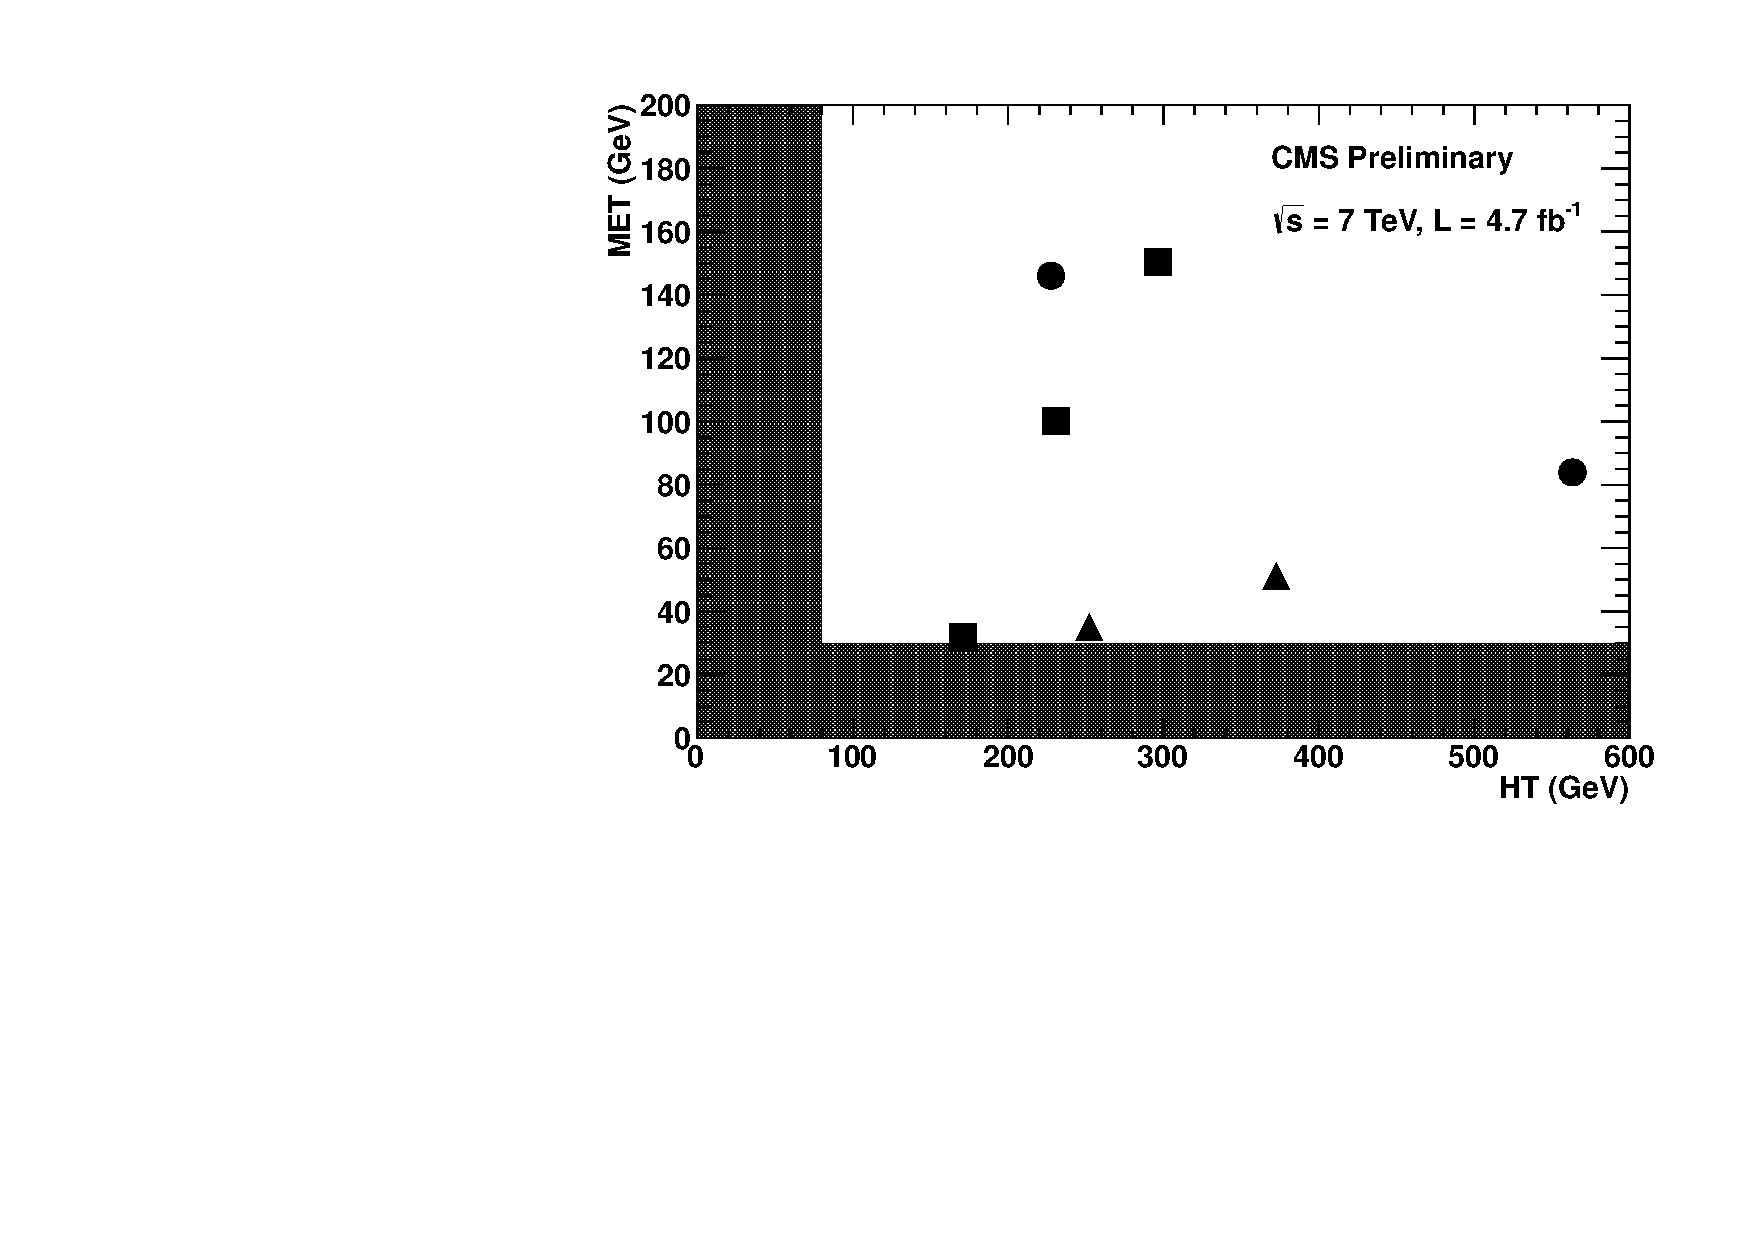
\includegraphics[width=0.48\linewidth]{figs/MetVsHt.pdf}
\caption{\label{fig:htvsmet}
Distribution of \met~~vs. $H_T$ for the 10 events in the baseline region: $H_T > 80$ GeV; $ee$ events: circles; $e\mu$ events: squares; $\mu\mu$ events: triangles.}
\end{center}
\end{figure}

\begin{figure}[h]
\begin{center}
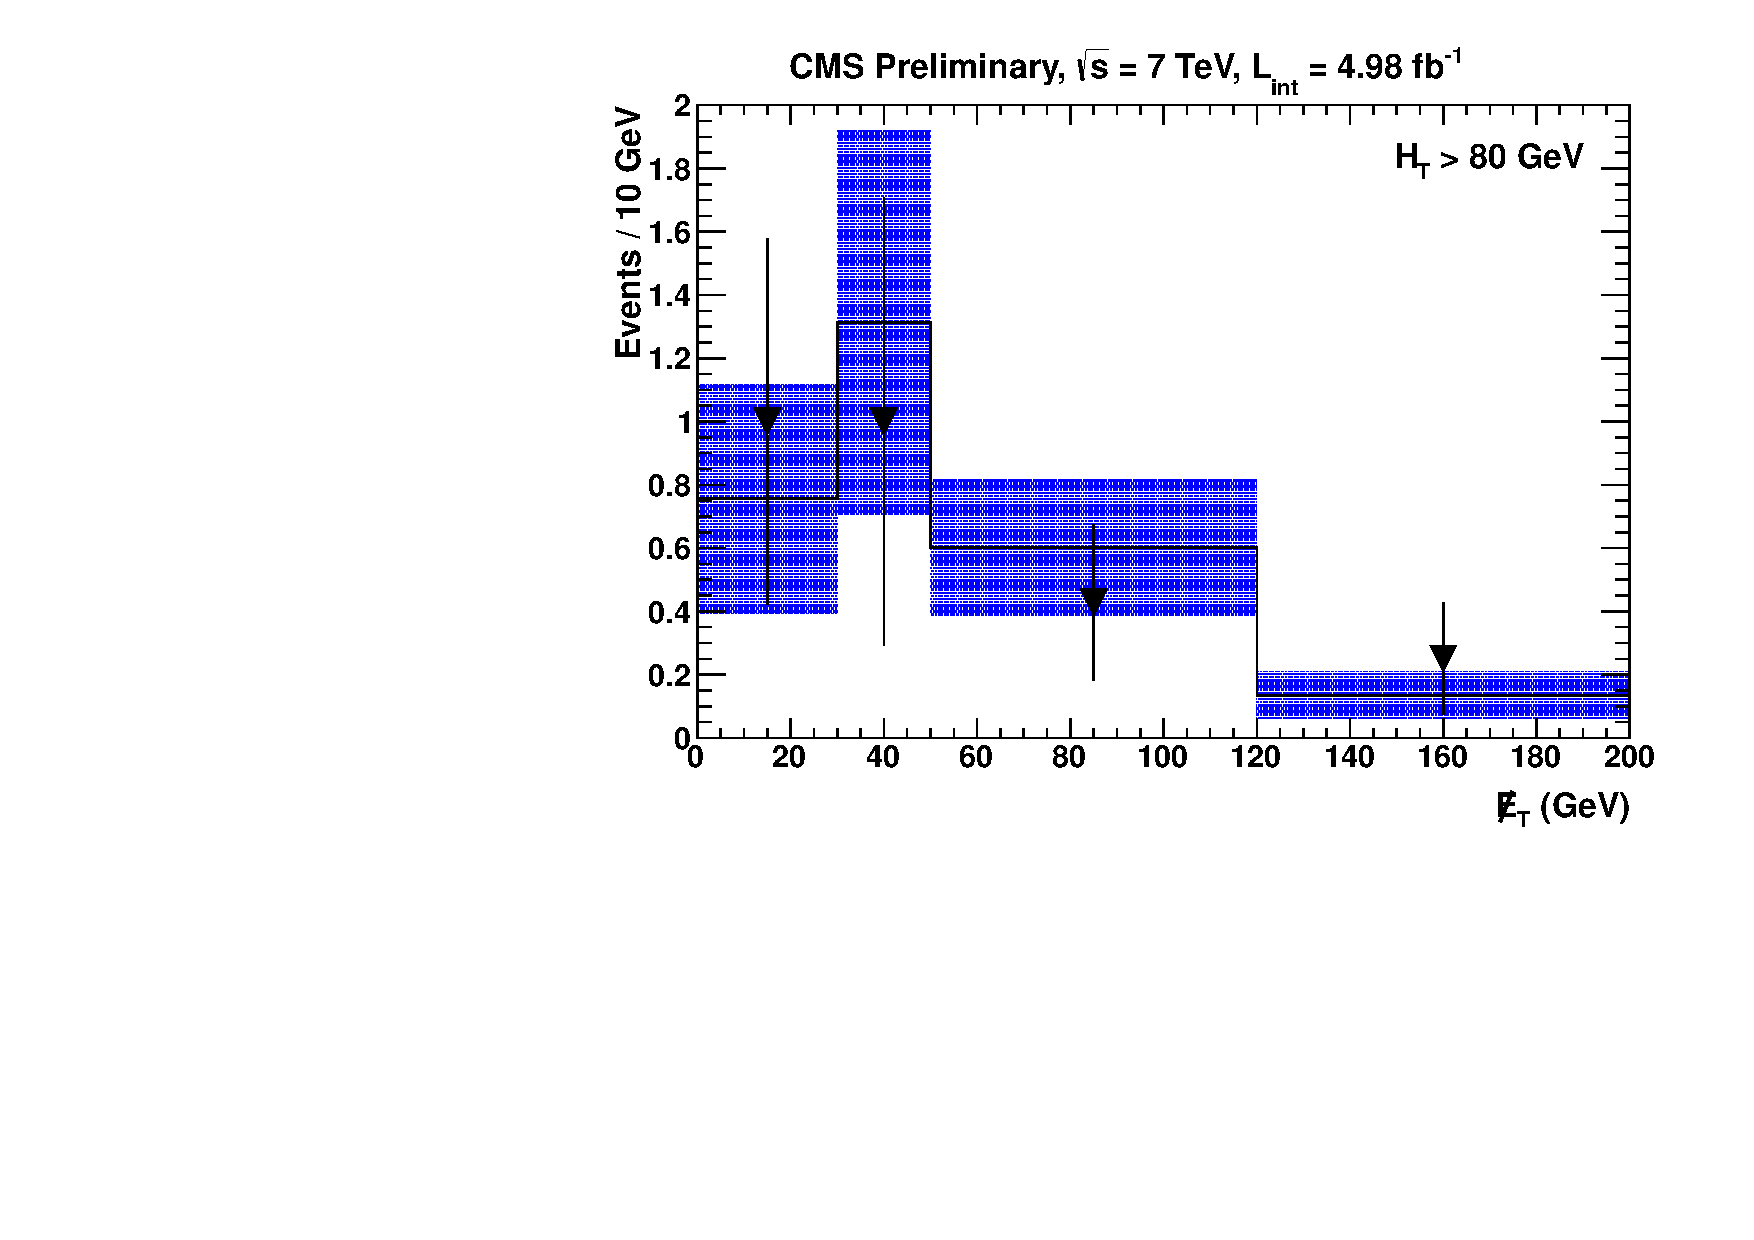
\includegraphics[width=0.48\linewidth]{figs/Met.pdf}
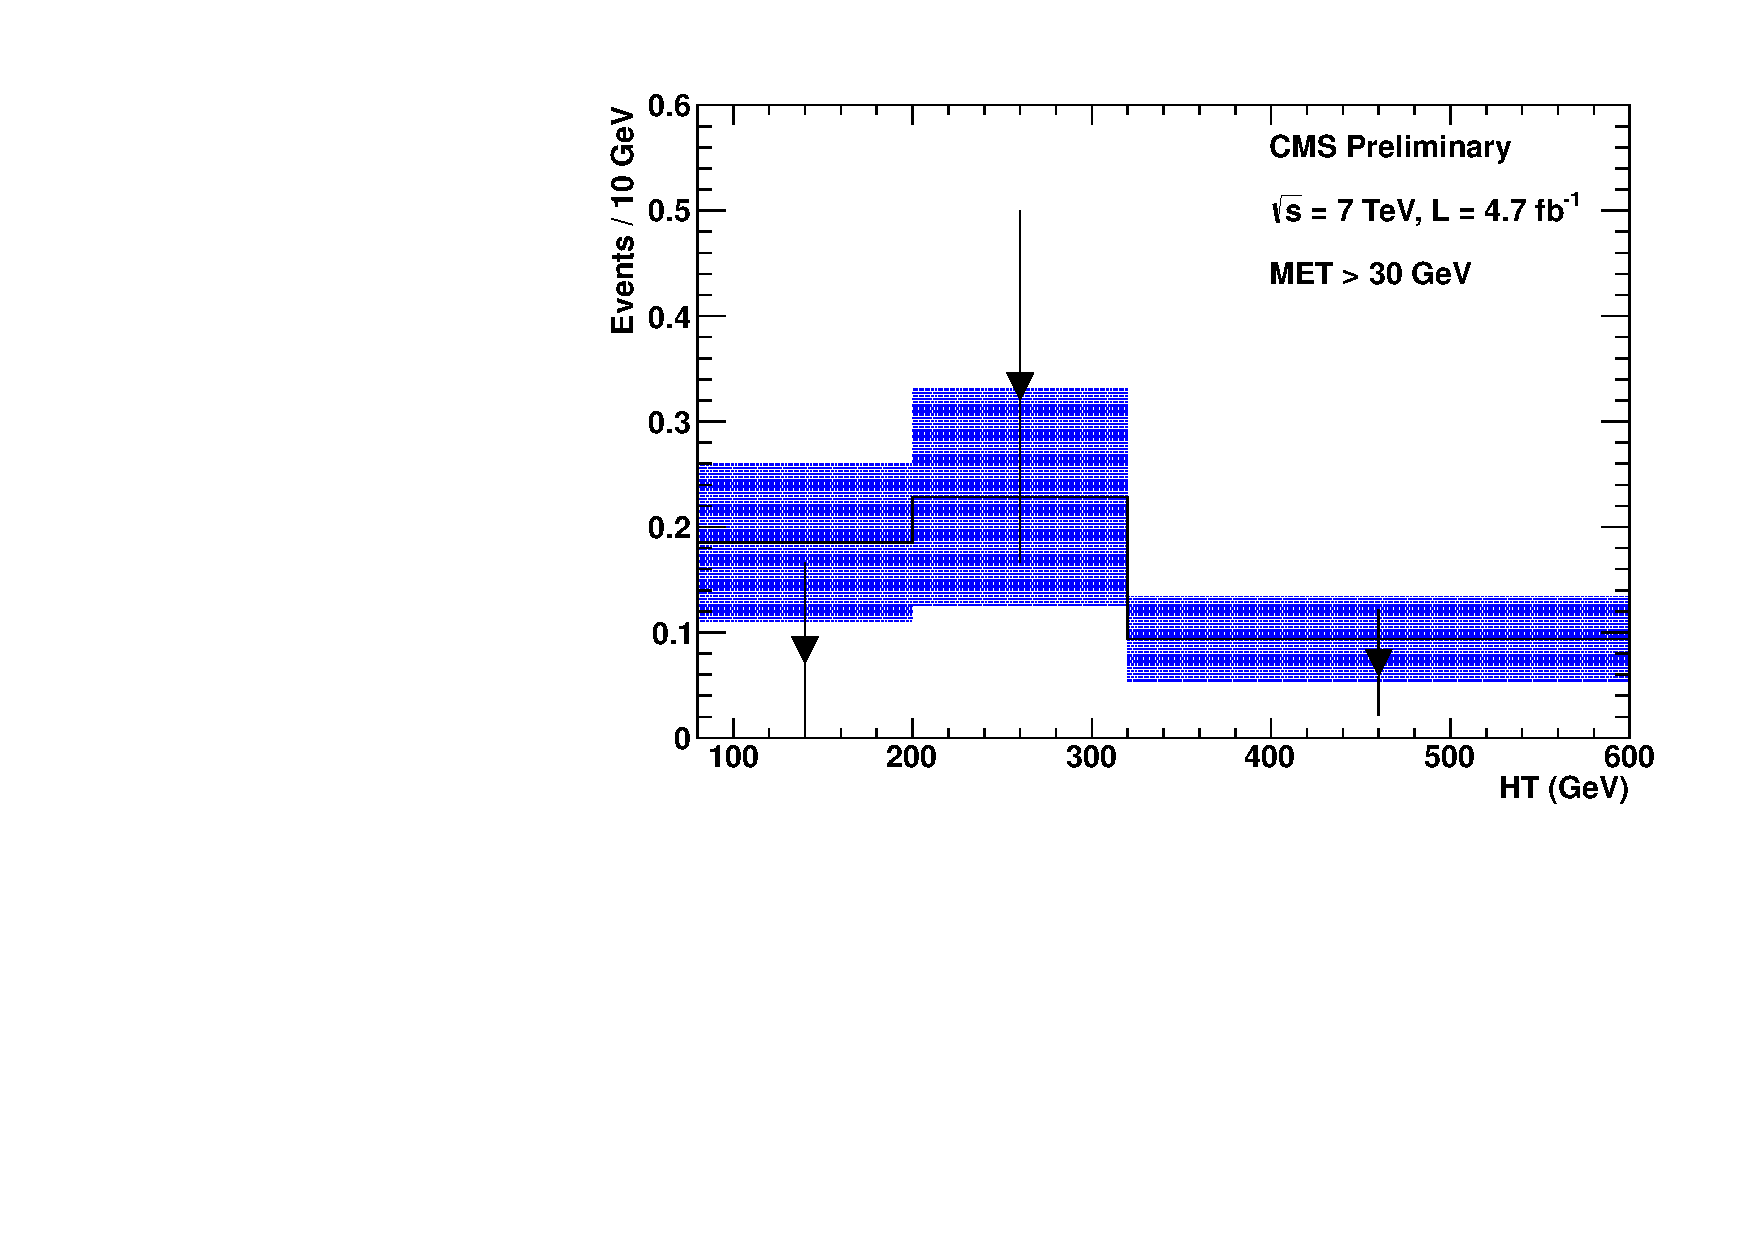
\includegraphics[width=0.48\linewidth]{figs/Ht.pdf}
\caption{\label{fig:htmet}
\met~~and $H_T$ distribution for the events in the baseline region (points).
Also shown as a histogram is the result of the background prediction.
The shading around the histogram represents the uncertainty
in the background prediction.}
\end{center}
\end{figure}


 





\section{Discussion of backgrounds}
\label{sec:bkgtypes}

As shown in Section~\ref{sec:yields}, the SM background to this study is dominated 
by \ttbar events. The contribution from single-top, diboson production ($WZ, ZZ$), 
is small. The diboson backgrounds will be estimated from Monte Carlo. 
The Monte Carlo acceptances for these processes will be corrected for differences between 
data and Monte Carlo lepton identification and trigger efficiencies, as determined using 
the tag-and-probe method.

We study the same sign dileptons for the \ttbar background based on their origin.
The dominant source of dileptons in \ttbar events are produced via, $t \rightarrow W b$; where 
$W \rightarrow \ell \nu $. We classify them as follows, based on truth matched to their ``parents'':

\begin{itemize}
\item Type-I: both leptons originate from real $W$ (including $W \rightarrow \tau \rightarrow \ell$) bosons, one with mis-reconstructed charge.
\item Type-II a): one of the leptons is from a real $W$ and the other originates from heavy flavor sources ($b, c$).
\item Type-II b): one of the leptons is from a $W$ and the other is a fake lepton.
\item Type-III: both leptons are fakes or from heavy flavor sources.
\end{itemize} 

\begin{figure}[htb]
\begin{center}
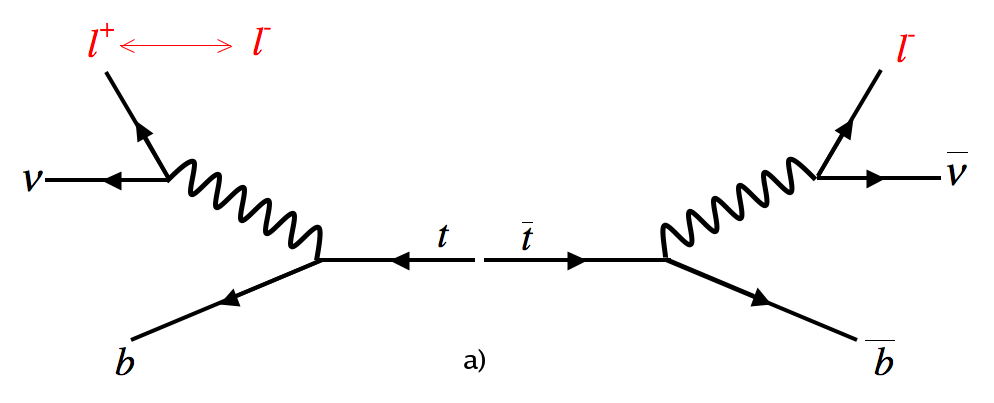
\includegraphics[width=0.32\linewidth, height=0.2\linewidth]{figs/feyntypeI.png}
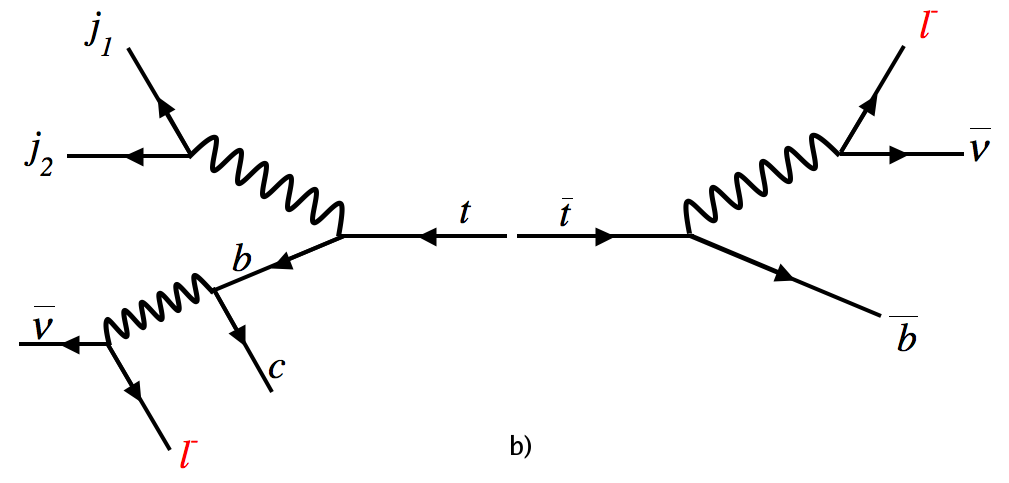
\includegraphics[width=0.32\linewidth, height=0.2\linewidth]{figs/feyntypeIIa.png}
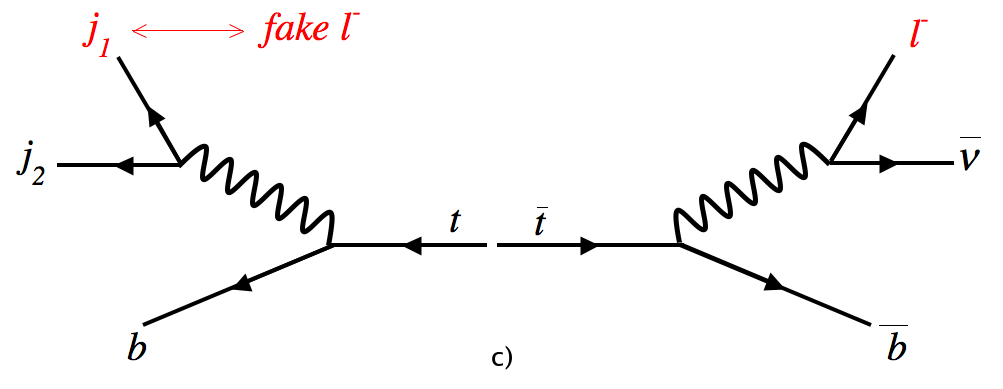
\includegraphics[width=0.32\linewidth, height=0.2\linewidth]{figs/feyntypeIIb.png}
\caption{ Classification of same sign dileptons from \ttbar decays. a) lepton from $W$ with mis-reconstructed charge; 
b) one of the lepton is from $W$, the other originating from heavy flavor sources; c) one of the lepton is from $W$,
and the other is a fake lepton. \label{fig:fakeOrigin}}
\end{center}
\end{figure}

Figure~\ref{fig:fakeOrigin} illustrates contribution from different types in \ttbar decays. The MC 
expectations of these contributions are given in Table~\ref{tab:fakeOrigin}.

\begin{table}[hbt]
\begin{center}
\begin{tabular}{|l|c|c|c|c|c|c|}\hline
Same Sign Leptons & Total & 	 Type-I &  Type-II & Type-II a) & Type-II b) & Type-III \\ \hline

$ee$ & 0.44$\pm$0.14 & 0.09$\pm$0.06 & 0.35$\pm$0.12 & 0.17$\pm$0.09 & 0.17$\pm$0.09 & 0.00$\pm$0.00 \\
$\mu\mu$ & 0.13$\pm$0.08 & 0.00$\pm$0.00 & 0.13$\pm$0.08 & 0.13$\pm$0.08 & 0.00$\pm$0.00 & 0.00$\pm$0.00 \\
$e\mu$ & 0.39$\pm$0.13 & 0.13$\pm$0.08 & 0.26$\pm$0.11 & 0.26$\pm$0.11 & 0.00$\pm$0.00 & 0.00$\pm$0.00 \\
total & 0.96$\pm$0.21 & 0.22$\pm$0.10 & 0.74$\pm$0.18 &	0.57$\pm$0.16 &	0.17$\pm$0.09 &	0.00$\pm$0.00 \\ \hline

\end{tabular}
\caption{ Expected number of \ttbar events of various types in 100 pb$^{-1}$ of integrated luminosity. Uncertainties are from MC statistics.\label{tab:fakeOrigin}}
\end{center}
\end{table}

It is interesting to note the following:
\begin{itemize}
\item Approximately $20 \%$, of the contribution is from Type-I (Charge mis-identification).
\item Almost all of the charge mis-identification is from electrons, in $ee$ and $e\mu$ channel.
\item The bulk of the \ttbar contribution in our event selection is from Type-II. The dominant among them 
is due to heavy flavor sources ($\sim 60 \%$)
\item No events with two fake leptons (Type-III) are expected within 100 pb$^{-1}$.
\end{itemize} 

In the following sections, we will briefly describe two different data driven approaches to 
estimate these contributions. The Type-I contribution will be estimated using the ``charge-flip rate'' described below, 
whereas the Type-II part will be estimated using the lepton fake rate method~\cite{fakelep}.




\section{Estimation of Charge Mis-Identification (Type-I)}
\label{sec:chargemisid}

In order to understand the Type-I background, we need to know the 
probability as a function of $P_T$ and $\eta$ for an electron
to have its charge misassigned (flipped).  We called this 
probability the ``charge-flip rate'', $P_{ChargeFlip}$.


The sample of $Z \to ee$ is an ideal sample to measure the charge-flip rate.
However, the $P_T$ range of electrons from $Z$ decays is limited
to (roughly) 20 GeV $< P_T <$ 60 GeV, while we need the flip-rate
down to 10 GeV and up to higher momenta.
Our plan then is to measure $P_{chargeFlip}$ from $Z$ data in the 
accessible $P_T$ range;  we will then compare 
the $P_{chargeFlip}$ from $Z$ data with the $P_{chargeFlip}$ from 
Monte Carlo using a single electron gun.  In the analysis we will
use the Monte Carlo flip rate, possibly adjusted if we find that
data and Monte Carlo do not agree


In this Section we demonstrate that we are able to extract 
$P_{chargeFlip}$ from a Monte Carlo Drell Yan sample, and that
this flip rate agrees with the flip rate from a 
single electron gun.  The analysis described here is based on 
a dielectron sample within the $Z$ mass region
($76 < m_{ee} < 106 $ GeV).   No opposite sign requirement is 
made.  Both electrons must pass all the identification and isolation
criteria described in Section~\ref{sec:eventselection}.



\subsection{Measurement of charge-flip rate on $Z$ events}

We define the charge-flip rate as

\begin{equation}
P_{ChargeFlip} = \frac{N_{Wrong}(P_T, |\eta|)}{N_{Total}(P_T, |\eta|)}
\end{equation}

where $N_{Wrong}(P_T, |\eta|)$ is the number of wrongly charged electrons  
and $N_{Total}(P_T, |\eta|)$ is 
the total number of electrons in the sample. We select events with same sign $(SS)$ 
and opposite sign $(OS)$ dielectrons within the $Z$ mass range, with both electrons passing the 
selection described in Section~\ref{sec:electron}.

We determine $P_{ChargeFlip}$ in two steps.  In the first step we limit ourselves
to the barrel region, $|\eta| < 1.0$, where we expect $P_{ChargeFlip}$ to have 
a small $\eta$ dependence.  Thus, we select $Z \to ee$, same sign (SS) as well as
opposite sign (OS), with both electrons in the barrel.  
We construct two $P_T-|\eta|$
distributions, one for electrons in the SS sample and 
one for electrons in the OS samples.  Neglecting the small 
probability of double charge flips, the OS distribution will contain only
electrons with the correct charge assignment, while the SS distribution
will contain a 50-50 admixture of charge flipped and non-charge flipped
electrons.  Then, 
the number of wrongly charged electrons in the barrel as a function
of $P_T$ and $|\eta|$ is obtained as

\begin{equation}
  N_{Wrong}(P_T, |\eta|) = SS(P_T, |\eta|) - k * OS(P_T, |\eta|) 
\end{equation}

The normalization $k$ is given by the ratio of SS and OS events.
The charge-flip rate in the barrel is then obtained by dividing 
$N_{Wrong}(P_T, |\eta|)$ by the total number of electrons as a 
function of $P_T$ and $|\eta|$.

Once $P_{ChargeFlip}$ in the barrel has been determined, the second step
of the procedure is to extend the measurement to higher rapidities 
($|\eta|>1$).  This is done using $Z \to ee$, OS as well as SS, with 
one electron of $|\eta|<1$ and one electron of $|\eta|>1$.  
$P_{ChargeFlip}$ for $|\eta|>1$ is determined by taking the ratio
of the $P_T-|\eta|$ distributions of electrons with 
$|\eta|>1$ in the SS sample to the total.  A correction needs to 
be applied to account for the events with the charge of the
$|\eta|<1$ flipped.  This is done using the  $P_{ChargeFlip}$
for $|\eta|<1$ determined in the first step.


\begin{figure}[htb]
\begin{center}
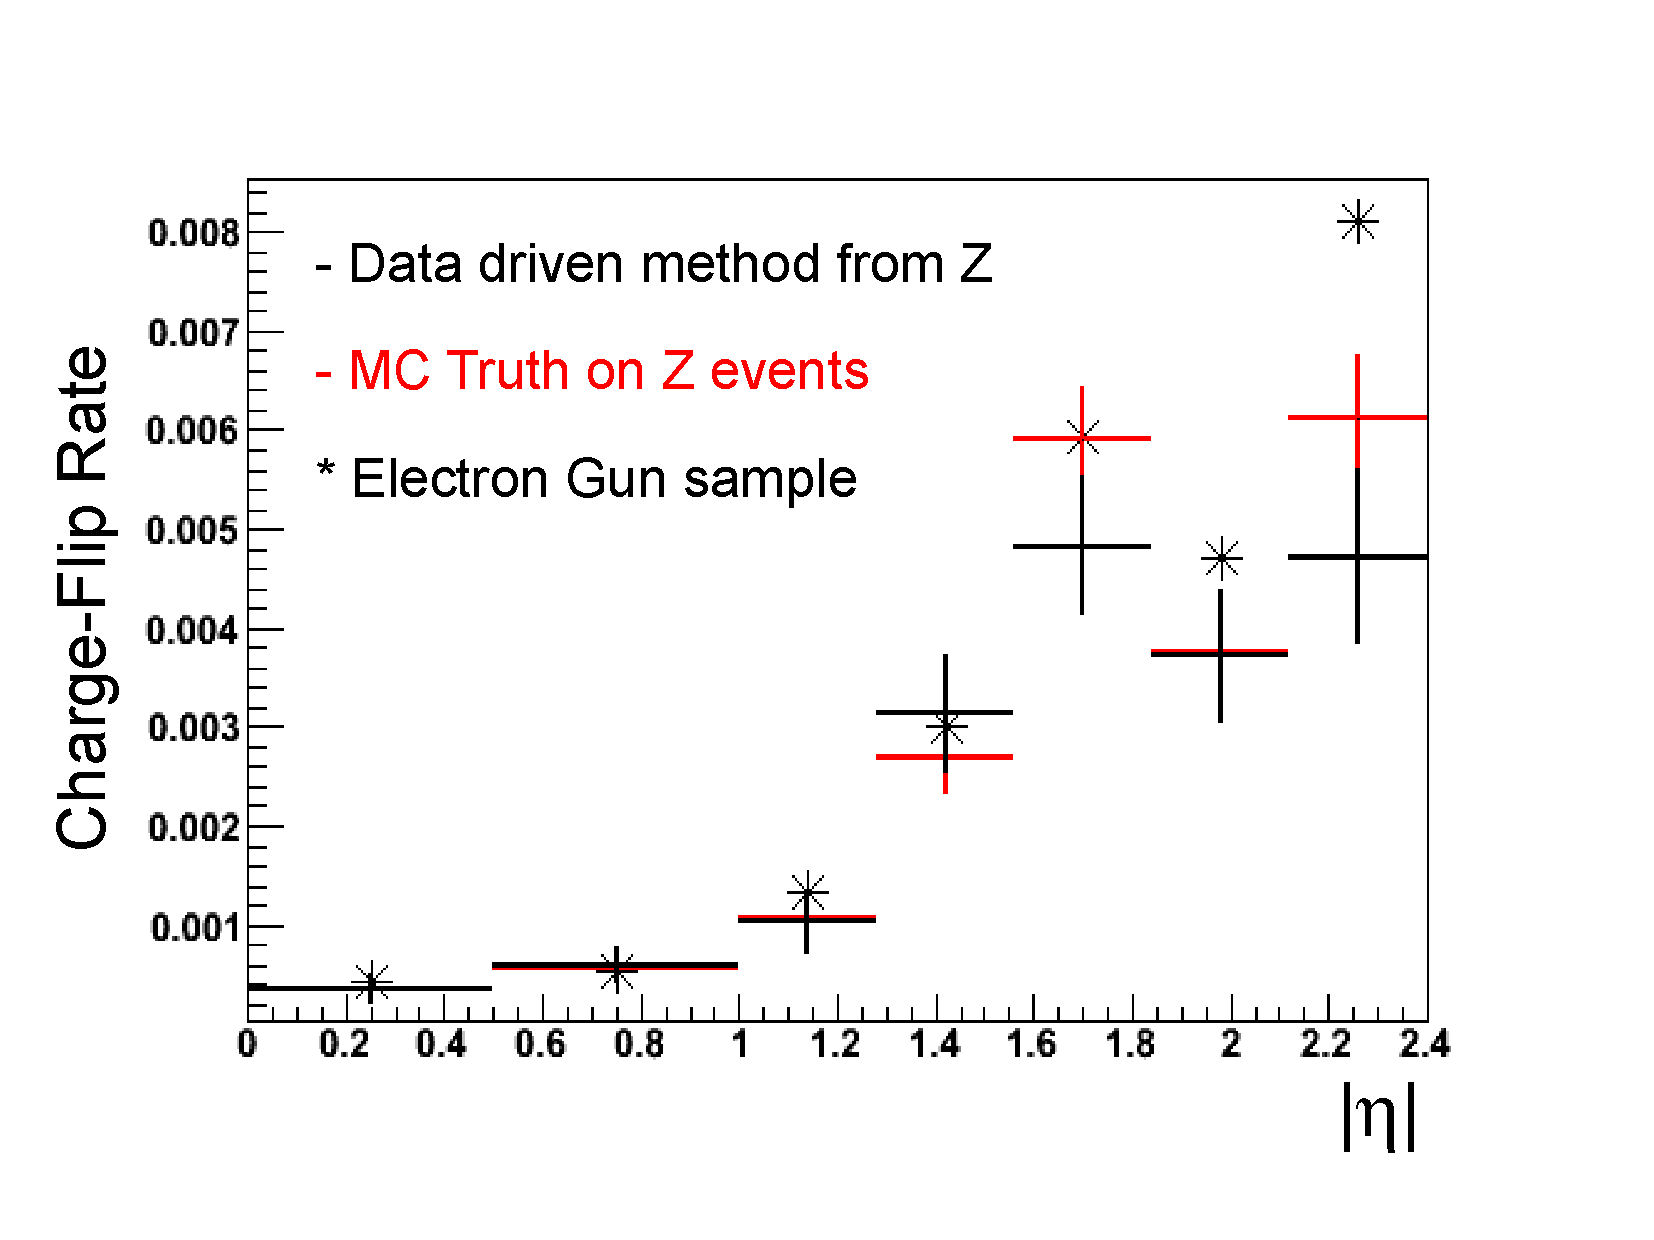
\includegraphics[width=0.7\linewidth]{figs/fr_rate.pdf}
\caption{Charge-flip rate as a function $|\eta|$ for the ``electron gun'' sample (star) compared with 
distributions using data driven method from $Z$ (black histograms) as well as truth matched $Z$ events 
(red histogram).
The integrated uminosity of the $Z$ sample is about 300 pb$^{-1}$.  
\label{fig:charge_fliprate}}
\end{center}
\end{figure}


It is important to verify that this procedure yields the correct 
charge-flip rate.  To this end, in Figure~\ref{fig:charge_fliprate}
we compare three flip rates as a function of $|\eta|$ and integrated
over $P_T$:
\begin{enumerate}
\item The flip rate obtained from the $Z$ sample using the two-step
procedure outlined above.
\item The flip rate obtained from the $Z$ sample using MC truth.
\item The flip rate obtained from the single electron gun, weighted by the
$P_T-\eta$ distribution of electrons in the $Z$ sample.
\end{enumerate}
The three distributions agree quite well. This demonstrates that 
we are able to measure the flip rate from the data in the $P_T$
region covered by $Z \to ee$. 


\subsection{Application of charge-flip rate to our analysis}

We now perform a test of the charge flip prediction on \ttbar MC events by relaxing cuts on \met and jets. The test is meant
to demonstrate that the charge-flip rate as determined from the ``electron gun'' sample can be applied
to \ttbar events. Dilepton events are selected without any \met and jet cuts using an integrated 
luminosity of 100 pb$^{-1}$. The observed event yield is obtained by selecting same sign dielectron events.
In order to get the estimation we use the following procedure:

\begin{itemize}
\item Select opposite sign dielectrons using the standard selection.
\item Obtain the $P^1_{ChargeFlip}$ and  $P^2_{ChargeFlip}$ for each electron for a given $p_T$ and $\eta$.
We use the charge-flip rate from the electron gun.
\item Assuming either of the electrons can flip signs, the flip probability is given by $ F = P_{ChargeFlip}/(1 - P_{ChargeFlip})$.
\item Weight each event by $weight * (F^1 + F^2)$.
\item Add up all of the weights
\end{itemize} 
Results of the Monte Carlo tests for event yields is given in Table~\ref{tab:ChFlip_Test}. From this study we 
can conclude that the charge-flip rate does a very good job of reproducing the rate of charge mis-identification
of electrons in \ttbar events.  
\begin{table}[hbt]
\begin{center}
\begin{tabular}{|l|c|}\hline
Sample & Event yield \\ \hline
\ttbar (Observed) & 2.4 $\pm$ 0.3 \\
\ttbar (Predicted) & 2.1 \\
\hline
\end{tabular}
\caption{ Monte Carlo test of the electron charge-flip rate.  Rates are normalized to 100 pb$^{-1}$ of integrated luminosity. \label{tab:ChFlip_Test}}
\end{center}
\end{table}

We are now ready to apply the charge-flip rate to our \ttbar sample after the full analysis selection. 
The same sign dilepton sample will have 
three different contributions from Type-I, Type-II and Type-III events. The results of the application of 
the procedure outlined above is summarized in Table~\ref{tab:ChFakePredict}.
\vspace{2mm}
\begin{table}[hbt]
\begin{center}
\begin{tabular}{|l|c|c|c|c|c|c|}\hline
Same Sign leptons & Total &      Type-I &  Type-II & Type-II a) & Type-II b) & Type-III \\ \hline
$ee$ (predicted) 	 & 0.05 & 	0.05 &	0.00 &	0.00 &	0.00 &	0.00 \\
$\mu\mu$ (predicted)     & 0.00 &	0.00 &	0.00 &	0.00 &	0.00 &	0.00 \\
$e\mu$ (predicted)	 & 0.07 &	0.07 &	0.00 &	0.00 &	0.00 &	0.00 \\
total (predicted) 	 & 0.12 &	0.12 &	0.00 &	0.00 &	0.00 &	0.00 \\
\hline
\end{tabular}
\caption{ The number of events predicted using charge-flip rate in \ttbar events for various types. Rates are normalized 
to 100 pb$^{-1}$.\label{tab:ChFakePredict}}
\end{center}
\end{table}

Using Table~\ref{tab:fakeOrigin} as observed and Table~\ref{tab:ChFakePredict} as the 
prediction, we find that the charge-flip method predicts the bulk of the Type-I events.
Out of a total of $0.22 \pm 0.10$ (roughly corresponds to 5 MC events) expected events, we predict 
$0.12$ ($\approx 3$) events in 100 pb$^{-1}$. As expected,
the method does not predict any contribution from Type-II events. 
We consider the agreement to be satisfactory.


\section{Data driven Method for Fake Lepton backgrounds (Type-II)}
\label{sec:leptonfake}

In this analysis, the primary source of events are from Type-II category. 
As shown in Table~\ref{tab:fakeOrigin}, approximately 3/4 of these events are expected to be from 
heavy flavor sources, while the remainder is from
fake leptons (Type-II b)). This means that one needs to be careful in defining the lepton fake rates
to make sure they predict both sources of fakes with sufficient accuracy.

In Reference~\cite{fakelep} we described a data-driven method to predict the fake 
background in a dilepton analysis. This method is also applied by us in  
the WW~\cite{ww} as well as \ttbar ~\cite{ttbar} analyses. Here we briefly
summarize the method, and apply it to the same sign dilepton study.

\subsection{The fake rate definition}
\label{subsec:fakeratedef}

The method starts by defining a fake rate ($FR$) measured in QCD events. We use 
the Pythia QCD samples with $\hat{P_T} > 30, 80 $ GeV. The fake rate is defined as 
the probability for a lepton passing loose cuts (Fakeable Object, $FO$) to pass the 
analysis cuts as a function of $p_T$ and $\eta$. The measured probability is then applied to 
dilepton candidates passing loose cuts to obtain a prediction to the fake lepton contribution. 
The details of the applications of the $FR$ are given in Section~\ref{subsec:fakerateapplication}. 

Fakeable Objects are defined as follows:

\begin{itemize}
\item Electron Fakeable Object, $eFO$:
\begin{itemize}
\item GSFElectron with $p_T > 10$ GeV;
\item $|\eta| < 2.4$;
\item No reconstructed muon with $\Delta R < 0.1$;
\item Electron ID and Conversion rejection defined in Section~\ref{sec:electron} as well as veto used in Section~\ref{sec:gsfctf};
\item Iso $<$ 0.4, where Iso=Sum/Max(20 GeV, $P_T$), and Sum = tkIso + hcalIso +  Max(0 GeV, ecalIso - 2 GeV).
\end{itemize} 

\item Muon Fakeable Object, $\mu FO$:
\begin{itemize}
\item Global and Tracker Muon with $p_T > 10$ GeV;
\item $|\eta| < 2.4$;
\item Global fit $\chi^2 /$ndof $ < 20 $;
\item $|d_0| < 200~\mu m$ (from silicon track, corrected for beamspot);
\item Iso $<$ 0.4, where Iso=Sum/Max(20 GeV, $P_T$), and Sum = tkIso + hcalIso +  ecalIso.
\end{itemize} 
\end{itemize} 

The $FR$ for electrons and muons are determined from the QCD sample.
% are shown in Figure.xx [Need a figure]
The $FR$ does not give a direct measure for an absolute lepton fake rate. It is the probability for a
fake lepton passing loose identification requirements as well as isolation to also pass a tighter
selection. 

\subsection{Application of lepton fake rate to our analysis}
\label{subsec:fakerateapplication}

We evaluate the $FR$ in \ttbar Monte Carlo events. This test is meant to check if the 
$FR$ as determined from the QCD events can be applied to \ttbar. In order to perform this test we 
define the following four event selections:

\begin{itemize}
\item \ttbar $\rightarrow Wb Wb \rightarrow \mu + e$  $ \nu \nu b b$:
\begin{itemize}
  \item Require a global muon with $p_T > 10$ GeV, truth matched to $W \rightarrow \mu$.
  \item Require a same sign electron that passes all the standard identification and isolation requirements. 
\end{itemize} 

\item \ttbar $\rightarrow Wb Wb \rightarrow \mu + (eFO \times FR)$  $ \nu \nu b b$:
\begin{itemize}
  \item Require a global muon with $p_T > 10$ GeV, truth matched to $W \rightarrow \mu$.
  \item Require a same sign $eFO$; weight each event by the $FR$ for the corresponding $eFO$.
\end{itemize} 

\item \ttbar $\rightarrow Wb Wb \rightarrow e + \mu  $  $ \nu \nu b b$:
\begin{itemize}
  \item Require an electron with $p_T > 10$ GeV, truth matched to $W \rightarrow e$.
  \item Require a same sign muon that passes all the standard identification and isolation requirements. 
\end{itemize} 

\item \ttbar $\rightarrow Wb Wb \rightarrow e + (\mu FO \times  FR)$  $ \nu \nu b b$:
\begin{itemize}
  \item Require an electron with $p_T > 10$ GeV, truth matched to $W \rightarrow e$.
  \item Require a same sign $\mu FO$; weight each event by the $FR$ for the corresponding $\mu FO$.
\end{itemize} 
\end{itemize} 

\begin{table}[hbt]
\begin{center}
\begin{tabular}{|l|c|}\hline
Sample & Event yield \\ \hline
\ttbar with $\mu + e$ (Observed) & 2.1 $\pm$ 0.3 \\
\ttbar with $\mu + (eFO \times FR)$ (Predicted) & 2.9 \\
\hline
\end{tabular}
\caption{ Monte Carlo test of the electron fake rate using 100 pb$^{-1}$ of integrated luminosity. The uncertainty is from Monte Carlo statistics.\label{tab:EleFR_Test}}
\end{center}
\end{table}
\begin{table}[hbt]
\begin{center}
\begin{tabular}{|l|c|}\hline
Sample & Event yield \\ \hline
\ttbar with $e + \mu$ (Observed) & 2.4 $\pm$ 0.3 \\
\ttbar with $e + (\mu FO \times FR)$ (Predicted) & 2.7 \\
\hline
\end{tabular}
\caption{ Monte Carlo test of the muon fake rate using 100 pb$^{-1}$ of integrated luminosity. The uncertainty is from Monte Carlo statistics.\label{tab:MuonFR_Test}}
\end{center}
\end{table}

The Monte Carlo test for the electron $FR$ consists of comparing event yields and distributions for 
$\mu + e $ and $\mu + (eFO \times FR)$. Similarly, for muon $FR$ it consists of comparing event yields 
and distributions for $ e + \mu$  and $e + (\mu DO \times FR)$. 
Results of the Monte Carlo tests for event yields are given in Tables~\ref{tab:EleFR_Test} and~\ref{tab:MuonFR_Test}.
The uncertainties are from the MC statistics. From these studies we conclude that the QCD $FR$ parametrization 
does a good job of reproducing the rate of fake electrons and muons in \ttbar events.

In order to obtain a prediction of the fake contribution to our analysis, we proceed in the following way:
\begin{itemize}
\item Select lepton $+ FO$ events where
\begin{itemize}
  \item one of the leptons passes all the standard identification and isolation requirements.
  \item the other lepton is a $FO$ but fails the standard identification and isolation requirements.
\end{itemize} 
\item The event passes all the standard kinematical cuts as outlined in Section~\ref{sec:eventselection}.
\item Weigh each event by $FR/(1 - FR)$, where $FR$ is the fake rate for the $FO$ under consideration.
\item Add up all the weights.
\end{itemize} 

\vspace{2mm}
\begin{table}[hbt]
\begin{center}
\begin{tabular}{|l|c|c|c|c|c|c|}\hline
Same Sign leptons & Total &      Type-I &  Type-II & Type-II a) & Type-II b) & Type-III \\ \hline
$ee$ (predicted) &	0.21 &	0.01 &	0.20 &	0.15 &	0.05 &	0.00 \\
$\mu\mu$ (predicted) &	0.10 &	0.00 &	0.10 &	0.09 &	0.01 &	0.00 \\
$e\mu$ (predicted) &	0.31 &	0.01 &	0.30 &	0.26 &	0.04 &	0.00 \\
total (predicted) &	0.62 &	0.02 &	0.60 &	0.50 &	0.10 &	0.00 \\
\hline
\end{tabular}
\caption{ The number of events predicted using lepton fake rate method in \ttbar events for various types. 
Rates are normalized to 100 pb$^{-1}$.\label{tab:LeptonFakePredict}}
\end{center}
\end{table}
 The results of the application of the procedure outlined above is summarized in Table~\ref{tab:LeptonFakePredict}. 
We conclude the following in comparison with the observed events from Table~\ref{tab:fakeOrigin}:


\begin{itemize}
\item We predict within $\sim 20 \%$ of the observed Type-II contributions.
\item Within Type-II, the contribution from events with heavy flavor sources are largely predicted ($\sim 88 \%$).
\item The method introduces an overestimate for the true leptons in Type-I. This is at $\sim 2 \%$ level, 
and is negligible compared to the associated statistical as well as systematic uncertainties.
\end{itemize}

\section{Application of the data driven methods to the SM and SUSY benchmark points}
\label{sec:application}
We apply the two data driven procedures to predict the backgrounds in the 
\ttbar-dominated SM sample. Table~\ref{tab:yieldsObsPre} shows the contribution 
of all SM background. The prediction and observation agree to within $\sim 30\%$.
\vspace{0.9mm}
\begin{table}[hbt]
\begin{center}
\renewcommand{\arraystretch}{1.2}
 {\footnotesize
\begin{tabular}{|l|c|c|c|c|c|c|c|c|}\hline
Same Sign Leptons & Total SM & \ttbar & tW & WZ & ZZ & WW & DY & Wjets \\ \hline
$ee$ (observed) & 0.45$\pm$0.14 & 0.44$\pm$0.14 & 0.00$\pm$0.00 & 0.00$\pm$0.00 & 0.01$\pm$0.01 & 0.00$\pm$0.00 & 0.00$\pm$0.00 & 0.00$\pm$0.00 \\
$ee$ (predicted) & 0.27 & 0.26 & 0.01 & 0.00 & 0.00 & 0.00 & 0.00 & 0.00 \\ \hline	
$\mu\mu$ (observed) & 0.17$\pm$0.08 & 0.13$\pm$0.08 & 0.00$\pm$0.00 & 0.03$\pm$0.02 & 0.01$\pm$0.01 & 0.00$\pm$0.00 & 0.00$\pm$0.00 & 0.00$\pm$0.00 \\
$\mu\mu$ (predicted) & 0.11 & 0.10 & 0.01 & 0.00 & 0.00 & 0.00 & 0.00 & 0.00 \\ \hline
$e\mu$ (observed) & 0.48$\pm$0.14 & 0.39$\pm$0.13 & 0.04$\pm$0.03 & 0.04$\pm$0.03 & 0.01$\pm$0.01 & 0.00$\pm$0.00 & 0.00$\pm$0.00 & 0.00$\pm$0.00 \\
$e\mu$ (predicted) & 0.39 & 0.38 & 0.01 & 0.00 & 0.00 & 0.00 & 0.00 & 0.00 \\ \hline	
total (observed) & 1.10$\pm$0.21 & 0.96$\pm$0.21 & 0.04$\pm$0.03 & 0.07$\pm$0.03 & 0.03$\pm$0.01 & 0.00$\pm$0.00 & 0.00$\pm$0.00 & 0.00$\pm$0.00 \\ \hline
total (predicted) & 0.77 & 0.74 & 0.03 & 0.00 & 0.00 & 0.00 & 0.00 & 0.00 \\ \hline
\end{tabular} }
\caption{Observed and predicted  number of SM events passing the event selection in 100 pb$^{-1}$ of integrated
luminosity. The uncertainties are from MC statistics.\label{tab:yieldsObsPre}}
\end{center}
\end{table}

We also apply both of these methods to a combination of SM and SUSY samples to derive the
prediction. Table~\ref{tab:yieldsSUSY} shows the contribution of observed and expected prediction to 
the sample. Typically, one would compare number of observed events with the prediction to look for excess 
in ``signal'' over the total background.

\vspace{0.9mm}
\begin{table}[hbt]
\begin{center}
%\small\addtolength{\tabcolsep}{-5pt}
\renewcommand{\arraystretch}{1.2}
{\footnotesize\addtolength{\tabcolsep}{-4pt} 
\begin{tabular}{|l|c|c|c|c|c|c|c|c|c|c|}\hline
Same Sign & SM+LM0 & SM+LM1 & SM+LM2 & SM+LM3 & SM+LM4 & SM+LM5 & SM+LM6 & SM+LM7 & SM+LM8 & SM+LM9 \\ \hline
Observed & 45.54$\pm$1.57 & 10.02$\pm$0.43 & 2.09$\pm$0.21 & 7.55$\pm$0.31 & 3.40$\pm$0.24 & 1.79$\pm$0.21 & 2.86$\pm$0.21 & 2.01$\pm$0.22 & 4.32$\pm$0.22 & 3.50$\pm$0.24 \\ \hline
Predicted & 4.10 & 1.26 & 0.83 & 1.24 &	0.91 &	0.81 &	0.84 &	0.83 &	1.03 &	1.00 \\ \hline
\end{tabular} }
\caption{Observed and predicted  number of SM and SUSY events passing the event selection in 100 pb$^{-1}$ of integrated
luminosity. The uncertainties are from MC statistics.\label{tab:yieldsSUSY}}
\end{center}
\end{table}

\section{Remarks on systematic uncertainties}
\label{sec:systematics}
The associated systematic uncertainties are not discussed in this document. We plan to measure
them in data. The expected dominant sources of systematic uncertainties 
are due to detector effects, effects 
of modeling of the contributing processes, and uncertainties of the data-driven background 
prediction methods.  Systematic uncertainties from the lepton selection, ID, and reconstruction efficiencies will be
estimated based on the corresponding systematics of the tag-and-probe method used to determine these efficiencies 
in $Z \rightarrow \ell \ell$ data. We will assess the uncertainty arising from the jet energy scale
using $\gamma/Z$ balance with jets. The uncertainties of the data-driven background estimate will be studied 
by determining a systematics on $FR$ and $P_{ChargeFlip}$ based on variations in the procedures for determining them in data.
%using 
%a measure of ``bias per lepton'' as a function of the either charge fake candidate in charge-flip rate or $FO$ in
%lepton fake rate selections. 
The current document focuses on demonstrating that these data driven methods work on Monte Carlo.
%reducing and measuring SM backgrounds using the aforesaid
%data driven methods.

\clearpage

\section{Conclusion}
\label{sec:conclusion}

We have assessed the sensitivity to mSUGRA of a generic signal characterized by two isolated, high $p_T$ leptons,
significant jet activity, and \met. We performed a scan of the mSUGRA $m_{0}-m_{1/2}$ parameter space and determined  
the expected excluded region in the case of no observed signal as well as the $5\sigma$ sensitivity reach for both SS
and OS dileptons, assuming integrated luminosities of 100 pb$^{-1}$ and 1 fb$^{-1}$. Our results indicate that we are sensitive to a
significant region of the mSUGRA parameter space which extends upon previous results from the Tevatron. 




\clearpage
\begin{thebibliography}{99}

\bibitem{cdf:recentSusy} {CDF Trilepton Search, 2009, CDF/PUB/EXOTIC/PUBLIC/9817};\\
{\small \tt http://www-cdf.fnal.gov/physics/exotic/r2a/20090521.trilepton\_3fb/Welcome.html}
%\bibitem{cdf:recentSusy1} {``Inclusive Search for Squark and Gluino Production in $p\bar{p}$ Collisions at $\sqrt{s}$ = 1.96-TeV'', Phys.Rev.Lett.102:121801, (2009).}
\bibitem{d0:recentSusy} {``Search for associated production of charginos and neutralinos in the trilepton final state using 2.3 fb$^{-1}$ of data'', Phys. Lett. B 680, 34 (2009).}
%\bibitem{d0:recentSusy1} {``Search for squarks and gluinos in events with jets and missing transverse energy using 2.1 fb$^{-1}$ of ppbar collision data at $sqrt(s)=1.96$ TeV'', 
%Phys. Lett. B 660 , 449 (2008).}

\bibitem{osnote} {``Data driven background estimate for a new physics search with opposite sign dileptons''}, CMS AN-2009/130.

\bibitem{ssnote} {``Data driven background study for new physics searches with same sign dileptons at $\sqrt{s} = 10 $ TeV''}, CMS AN-2009/138.

\bibitem{mcsusy}{\tt https://twiki.cern.ch/twiki/bin/viewauth/CMS/SUSYMCRequirements0911}.

\bibitem{fast10}{\tt https://twiki.cern.ch/twiki/bin/view/CMS/SUSY33XScan}.

\bibitem{ww} {``Prospects for measuring the $WW$ production cross section in $pp$ collisions at $\sqrt s = $10 TeV''}, CMS AN-2009/042 and PAS EWK-09-002.

\bibitem{ttbar} {``Expectations for observation of top quark pair production in the dilepton final state with the early CMS data''}, CMS AN-2009/050 and PAS TOP-09-002.

\bibitem{tcmet} {``Correcting Missing Transverse Energy Using Tracks``} CMS AN-2009/022.

\bibitem{conversionnote} {``Study of photon conversion rejection at CMS''}, CMS AN-2009/159.

\bibitem{glbtrk} {\tt https://hypernews.cern.ch/HyperNews/CMS/get/muon/258.html}.

\bibitem{muonid} {``Muon Identification in CMS''}, CMS AN-2008/098.

\bibitem{vplusj} {\tt https://twiki.cern.ch/twiki/bin/view/CMS/VplusJets}.

\bibitem{fakenote} {``Data-driven methods to estimate the electron and muon fake contributions to lepton analyses''}, CMS AN-2009/041.

\bibitem{cite:cousins} {``Evaluation of three methods for calculating statistical significance when incorporating a systematic uncertainty into a test of the background-only hypothesis for a Poisson process''} arXiv:physics/0702156 [physics.data-an]

\bibitem{cite:conway} {``Interval estimation in the presence of nuisance parameters. 1. Bayesian approach''} arXiv:physics/0409129v1 [physics.data-an]

\bibitem{lep:lepsusyreach}{LEP Susy working group: {\tt http://lepsusy.web.cern.ch/lepsusy/} }

\bibitem{bayes}{\tt http://arxiv.org/pdf/physics/0409129}

\bibitem{victor} {\tt http://arxiv.org/pdf/0906.5016}; \\
{\tt http://indico.cern.ch/contributionDisplay.py?contribId=2\&confId=39042}.

\bibitem{summer09}{\tt https://twiki.cern.ch/twiki/bin/view/CMS/SUSY31XProduction}.


\end{thebibliography}

\end{document}
